\documentclass[11pt,oneside]{book}

\usepackage[T1]{fontenc}
\usepackage[utf8]{inputenc}
\usepackage{lmodern}
\usepackage[letterpaper,margin=1in]{geometry}
\usepackage{microtype}
\usepackage{amsmath,amssymb,amsthm,mathtools}
\usepackage{bm}
\usepackage{booktabs,longtable,array}
\usepackage{graphicx}
\usepackage{enumitem}
\usepackage{xcolor}
\usepackage{tikz}
\usepackage{fancyhdr}
\usepackage{hyperref}
\usepackage[nameinlink,capitalise,noabbrev]{cleveref}

\hypersetup{
  colorlinks=true,
  linkcolor=blue!55!black,
  citecolor=green!40!black,
  urlcolor=blue!65!black,
  pdftitle={The Lambert W Function: Real Branches, Series, Asymptotics, Bounds, Algorithms, and Applications},
  pdfauthor={OpenAI}
}

\setcounter{tocdepth}{2}
\setcounter{secnumdepth}{3}
\allowdisplaybreaks
\setlist{nosep}

\setlength{\headheight}{14pt}
\pagestyle{fancy}
\fancyhf{}
\fancyhead[L]{\nouppercase{\leftmark}}
\fancyhead[R]{\thepage}
\renewcommand{\headrulewidth}{0.4pt}

\newtheorem{theorem}{Theorem}[chapter]
\newtheorem{proposition}[theorem]{Proposition}
\newtheorem{lemma}[theorem]{Lemma}
\newtheorem{corollary}[theorem]{Corollary}
\newtheorem{claim}[theorem]{Claim}
\theoremstyle{definition}
\newtheorem{definition}[theorem]{Definition}
\newtheorem{example}[theorem]{Example}
\newtheorem{algorithm}[theorem]{Algorithm}
\newtheorem{exercise}[theorem]{Exercise}
\theoremstyle{remark}
\newtheorem{remark}[theorem]{Remark}
\newtheorem{warning}[theorem]{Branch warning}

\newcommand{\W}{W}
\newcommand{\Wz}{W_0}
\newcommand{\Wm}{W_{-1}}
\newcommand{\ee}{\mathrm e}
\newcommand{\ii}{\mathrm i}
\newcommand{\Log}{\operatorname{Log}}
\newcommand{\R}{\mathbb R}
\newcommand{\C}{\mathbb C}
\newcommand{\Z}{\mathbb Z}
\newcommand{\N}{\mathbb N}
\newcommand{\Res}{\operatorname*{Res}}
\newcommand{\Li}{\operatorname{Li}}
\newcommand{\sgn}{\operatorname{sgn}}
\newcommand{\bigO}{\mathcal O}
\newcommand{\littleo}{o}
\newcommand{\coeff}[2]{[z^{#1}]\,#2}
\newcommand{\stirlingone}[2]{\genfrac{[}{]}{0pt}{}{#1}{#2}}

\title{\Huge The Lambert $W$ Function\\[0.5em]
\Large Real Branches, Series, Asymptotics, Bounds, Algorithms, and Applications}
\author{A self-contained mathematical introduction}
\date{August 2026}

\begin{document}
\frontmatter
\hypersetup{pageanchor=false}
\maketitle
\cleardoublepage
\hypersetup{pageanchor=true}
\setcounter{page}{1}

\chapter*{Abstract}
\addcontentsline{toc}{chapter}{Abstract}
The Lambert $W$ function is the multivalued inverse of $w\mapsto w\ee^w$.
That definition is short, but its consequences reach from elementary equation
solving to combinatorics, differential equations, circuit theory, biochemical
kinetics, numerical analysis, and asymptotic inversion.  This article develops
the subject from first principles.  Special attention is paid to the two real
branches: the principal branch $W_0$ and the often omitted lower branch
$W_{-1}$.  We prove their domains, monotonicity, curvature, differential and
integral identities, Taylor and Puiseux series, logarithmic asymptotic
expansions, elementary bounds, and branch-safe iterative algorithms.  We also
derive representative applications rather than merely listing them.

The exposition assumes single-variable calculus and elementary power series.
More advanced tools---formal residues, Lagrange inversion, and complex branch
cuts---are introduced when needed and proved or explained in appendices.  The
attached numerical program independently checks the main expansions and
produces the figures in the article.  Material and perspectives from the
source archive include the canonical treatment of Corless, Gonnet, Hare,
Jeffrey, and Knuth; DLMF formulas; real-branch approximations of Barry and
coauthors and of Iacono and Boyd; bounds for $W_{-1}$ due to Chatzigeorgiou;
continued fractions of Corcino, Corcino, and Mezo; the guaranteed iteration
analysis of Loczi; and applications in electronics, kinetics, ecology, and
prime-number estimates.


\tableofcontents

\chapter*{How to read this article}
\addcontentsline{toc}{chapter}{How to read this article}
The quickest route is Chapters~\ref{ch:def}--\ref{ch:equations}, followed by
Chapters~\ref{ch:series}, \ref{ch:branchpoint}, and \ref{ch:asymptotics}.
Readers primarily interested in reliable computation can then jump to
Chapter~\ref{ch:numerics}.  Applications are collected in
Chapter~\ref{ch:applications}.

The notation $W(x)$ without a subscript is used only when the branch is either
irrelevant or explicitly fixed by context.  On the real axis, $W_0$ and
$W_{-1}$ are always written separately whenever two real values are possible.
This convention is not cosmetic: selecting the wrong branch can change a
physical time, concentration, or threshold by orders of magnitude.

\mainmatter

\chapter{Definition, geometry, and the two real branches}\label{ch:def}

\section{The inverse problem}

The ordinary logarithm solves the inverse problem for the exponential:
$\ee^w=x$ if and only if $w=\log x$.  The Lambert function solves the next
natural inverse problem, in which the unknown occurs both outside and inside
an exponential.

\begin{definition}[Lambert $W$ relation]
For $z\in\C$, the values of the Lambert $W$ relation are the complex numbers
$w$ satisfying
\begin{equation}\label{eq:defining}
  w\ee^w=z.
\end{equation}
Its single-valued branches are denoted $W_k(z)$, where $k\in\Z$.  Thus
\begin{equation}\label{eq:branchdef}
  W_k(z)\ee^{W_k(z)}=z
\end{equation}
wherever the branch $W_k$ is defined.
\end{definition}

The word ``relation'' matters over $\C$: just as the complex logarithm has
infinitely many values, the inverse of $w\ee^w$ has infinitely many branches.
Over $\R$, however, the geometry is particularly transparent.

\section{Complete classification of real solutions}

Let
\[
  f(w)=w\ee^w,\qquad w\in\R.
\]
Then
\begin{equation}\label{eq:fderivatives}
  f'(w)=\ee^w(1+w),\qquad f''(w)=\ee^w(2+w).
\end{equation}

\begin{theorem}[Real branches]\label{thm:realbranches}
The equation $w\ee^w=x$ has the following real solutions.
\begin{enumerate}[label=\textup{(\roman*)}]
\item If $x<-1/\ee$, there is no real solution.
\item If $x=-1/\ee$, there is exactly one real solution, $w=-1$.
\item If $-1/\ee<x<0$, there are exactly two real solutions:
\[
  -1<W_0(x)<0,\qquad W_{-1}(x)<-1.
\]
\item If $x=0$, the only finite real solution is $W_0(0)=0$; moreover
$W_{-1}(x)\to-\infty$ as $x\uparrow0$.
\item If $x>0$, there is exactly one real solution, $W_0(x)>0$.
\end{enumerate}
Consequently,
\begin{align*}
 W_0&:[-1/\ee,\infty)\longrightarrow[-1,\infty),\quad\text{strictly increasing},\\
 W_{-1}&:[-1/\ee,0)\longrightarrow(-\infty,-1],\quad\text{strictly decreasing}.
\end{align*}
\end{theorem}

\begin{proof}
The exponential is positive, so $f(w)$ has the same sign as $w$.  By
\eqref{eq:fderivatives}, $f'(w)<0$ for $w<-1$, $f'(-1)=0$, and $f'(w)>0$
for $w>-1$.  Hence $f$ decreases on $(-\infty,-1]$ and increases on
$[-1,\infty)$.  Its minimum is
\[
  f(-1)=-\ee^{-1}.
\]
Furthermore,
\[
 \lim_{w\to-\infty}w\ee^w=0^-,\qquad f(0)=0,
 \qquad\lim_{w\to+\infty}w\ee^w=+\infty.
\]
The intermediate value theorem and strict monotonicity on each interval now
give every assertion, including the ranges and monotonicity of the inverse
branches.
\end{proof}

\begin{figure}[htbp]
\centering
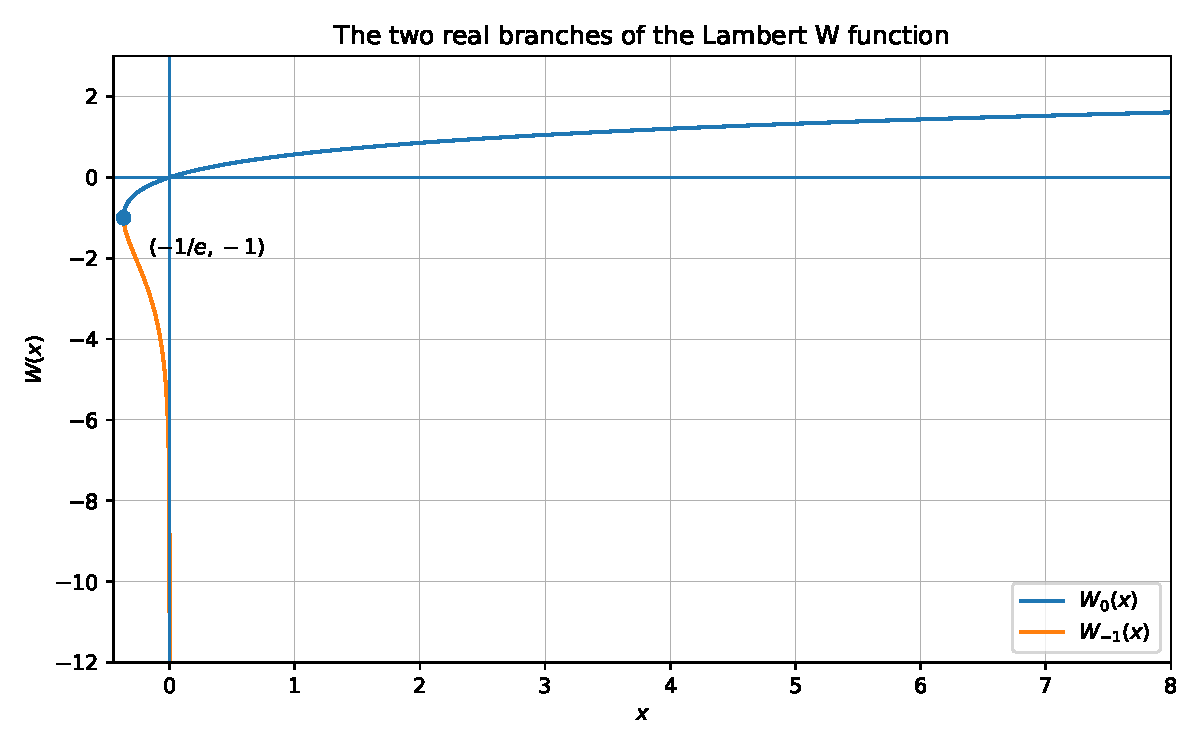
\includegraphics[width=0.9\textwidth]{fig_real_branches.pdf}
\caption{The two real branches.  They meet at the square-root branch point
$(-1/\ee,-1)$.  The lower branch tends to $-\infty$ as $x\uparrow0$.}
\label{fig:realbranches}
\end{figure}

\section{Immediate identities and their domains}

Whenever $w=W_k(z)$ is nonzero, the defining equation gives
\begin{equation}\label{eq:expW}
  \ee^{W_k(z)}=\frac{z}{W_k(z)},
  \qquad
  \ee^{-W_k(z)}=\frac{W_k(z)}{z}.
\end{equation}
At $z=0$ the first quotient has a removable singularity on $W_0$ because
$W_0(z)\sim z$.

Taking a logarithm is more delicate over $\C$, but on a fixed real branch
there is no ambiguity:
\begin{align}
 W_0(x)+\log W_0(x)&=\log x &&(x>0),\label{eq:logpositive}\\
 W_j(x)+\log\bigl(-W_j(x)\bigr)&=\log(-x)
 &&(-1/\ee\le x<0,\ j=0,-1).\label{eq:lognegative}
\end{align}

\begin{proposition}[Exact inversion of $t\mapsto t\ee^t$]\label{prop:branchselect}
For real $t$,
\begin{align}
 W_0(t\ee^t)&=t &&\text{if }t\ge-1,\label{eq:w0inverse}\\
 W_{-1}(t\ee^t)&=t &&\text{if }t\le-1.\label{eq:wm1inverse}
\end{align}
In particular, for $a>0$,
\begin{align}
 W_0(a\log a)&=\log a &&\text{if }a\ge\ee^{-1},\label{eq:alogaplus}\\
 W_{-1}(a\log a)&=\log a &&\text{if }0<a\le\ee^{-1}.
\label{eq:alogaminus}
\end{align}
\end{proposition}

\begin{proof}
The restrictions in \eqref{eq:w0inverse} and \eqref{eq:wm1inverse} place $t$
in the range of the stated inverse branch.  Since $t$ itself solves
$w\ee^w=t\ee^t$ and the inverse is unique on that range, the formulas follow.
Set $t=\log a$ for the last two identities.
\end{proof}

\begin{warning}
The unqualified formula $W(t\ee^t)=t$ is false.  For example,
$(-2)\ee^{-2}\in(-1/\ee,0)$ has two preimages.  One branch returns $-2$ and
the other returns the distinct number $W_0(-2\ee^{-2})\in(-1,0)$.
\end{warning}

\section{Special values}

Most Lambert values are transcendental-looking constants rather than familiar
numbers.  Exact values arise whenever the argument is deliberately written as
$t\ee^t$:
\[
 W_0(0)=0,
 \quad W_0(-1/\ee)=W_{-1}(-1/\ee)=-1,
 \quad W_0(\ee)=1,
 \quad W_0(2\ee^2)=2,
 \quad W_{-1}(-3\ee^{-3})=-3.
\]
The positive constant
\begin{equation}\label{eq:omega}
  \Omega=W_0(1)=0.567143290409783872999\ldots
\end{equation}
is called the \emph{omega constant}; it is the unique positive solution of
$\Omega\ee^\Omega=1$, equivalently $\Omega+\log\Omega=0$.

\begin{center}
\begin{tabular}{@{}rll@{}}
\toprule
$x$ & $W_0(x)$ & $W_{-1}(x)$ when real \\
\midrule
$-1/e$ & $-1.0$ & $-1.0$ \\
$-0.1$ & $-0.111832559158962965$ & $-3.57715206395729722$ \\
$0$ & $0.0$ & -- \\
$1$ & $0.567143290409783873$ & -- \\
$e$ & $1.0$ & -- \\
$10$ & $1.74552800274069938$ & -- \\
\bottomrule
\end{tabular}

\end{center}

\chapter{Putting equations into Lambert form}\label{ch:equations}

The main practical skill is not memorizing formulas but recognizing how to
create a product $u\ee^u$ in which the same transformed unknown appears in
both positions.

\section{A general affine--exponential equation}

\begin{theorem}[Affine factor times an exponential]\label{thm:affineexp}
Let $a,c,r\ne0$ and let $b,d$ be constants.  Every solution of
\begin{equation}\label{eq:affineexp}
  (ax+b)\ee^{cx+d}=r
\end{equation}
is of the form
\begin{equation}\label{eq:affineexpsolution}
  x=\frac1c W_k\!\left(\frac{cr}{a}
       \exp\!\left(\frac{cb}{a}-d\right)\right)-\frac ba,
\end{equation}
for a branch $k$ on which the displayed value is defined.  Conversely, every
such branch value solves \eqref{eq:affineexp}.
\end{theorem}

\begin{proof}
Set $u=ax+b$, so $x=(u-b)/a$.  Equation \eqref{eq:affineexp} becomes
\[
 u\exp\!\left(\frac ca u+d-\frac{cb}{a}\right)=r.
\]
Multiplying by $(c/a)\exp(cb/a-d)$ gives
\[
 \left(\frac ca u\right)\exp\!\left(\frac ca u\right)
 =\frac{cr}{a}\exp\!\left(\frac{cb}{a}-d\right).
\]
Apply the defining inverse relation, then substitute back
$u=ax+b$.  Reversing the algebra proves the converse.
\end{proof}

\begin{example}[A decay equation with two times]
Consider
\[
 (1-t)\ee^t=q,
\]
where $0<q<1$.  Set $u=t-1$.  Then $-u\ee^{u+1}=q$, so
\[
 t=1+W_k(-q/\ee).
\]
Because $-q/\ee\in(-1/\ee,0)$, there are two real formal values.  They
correspond to $W_0$ and $W_{-1}$.  A model that also requires $t\ge0$ or
$t\le1$ must use that extra information to select the physical value.
\end{example}

\section{Logarithmic--linear equations}

\begin{proposition}\label{prop:loglinear}
For $A,B\ne0$, positive solutions of
\begin{equation}\label{eq:loglinear}
 A\log x+Bx=C
\end{equation}
are
\begin{equation}\label{eq:loglinearsol}
 x=\frac AB W_k\!\left(\frac BA\ee^{C/A}\right),
\end{equation}
with exactly those branches that make the right-hand side positive and real.
\end{proposition}

\begin{proof}
Divide by $A$ and exponentiate:
$x\exp((B/A)x)=\exp(C/A)$.  Multiplication by $B/A$ creates the defining
product.  The converse follows by substitution.
\end{proof}

\section{The equation $x^x=a$}

For $x>0$, put $u=\log x$.  Then $x=\ee^u$ and
\[
 x^x=a
 \quad\Longleftrightarrow\quad
 x\log x=\log a
 \quad\Longleftrightarrow\quad
 u\ee^u=\log a.
\]
Hence
\begin{equation}\label{eq:xxa}
 x=\exp\bigl(W_k(\log a)\bigr)
   =\frac{\log a}{W_k(\log a)},
\end{equation}
where the quotient is interpreted by continuity at $a=1$.

\begin{theorem}[Number of positive solutions of $x^x=a$]\label{thm:xxa}
Let $a>0$.
\begin{enumerate}[label=\textup{(\roman*)}]
\item If $0<a<\ee^{-1/\ee}$, there is no positive solution.
\item If $a=\ee^{-1/\ee}$, the unique solution is $x=\ee^{-1}$.
\item If $\ee^{-1/\ee}<a<1$, there are exactly two positive solutions,
obtained from $W_0(\log a)$ and $W_{-1}(\log a)$ in \eqref{eq:xxa}.
\item If $a\ge1$, there is exactly one positive solution.
\end{enumerate}
\end{theorem}

\begin{proof}
The derivative of $g(x)=x\log x$ is $1+\log x$.  Thus $g$ decreases on
$(0,\ee^{-1})$, increases on $(\ee^{-1},\infty)$, and has minimum
$g(\ee^{-1})=-1/\ee$.  Exponentiating gives the corresponding minimum of
$x^x$, namely $\ee^{-1/\ee}$.  For $\log a\in(-1/\ee,0)$,
\Cref{thm:realbranches} supplies exactly two real values of $W$, and their
exponentials are the two positive solutions.  The remaining cases follow
from the same monotonicity.
\end{proof}

\section{The equation $x^y=y^x$}

For positive $x,y$ with $x\ne1$, the equation is equivalent to
\[
 \frac{\log y}{y}=\frac{\log x}{x}=:a.
\]
Solving $\log y=ay$ gives
\begin{equation}\label{eq:xyyx}
 y=-\frac{1}{a}W_k(-a),\qquad a=\frac{\log x}{x}.
\end{equation}
One branch reproduces $y=x$; when $0<a<1/\ee$ the other branch gives the
familiar nontrivial partner.  The branch point $a=1/\ee$ corresponds to
$x=y=\ee$.

\begin{example}
Take $x=2$.  Then $a=(\log2)/2$.  The branch satisfying
$W_k(-a)=-a x=-\log2$ gives $y=2$.  The other branch yields $y=4$, and indeed
$2^4=4^2$.
\end{example}

\section{Infinite power towers}

A convergent positive tower
\[
 T=x^{x^{x^{\cdot^{\cdot^{\cdot}}}}}
\]
must satisfy $T=x^T$.  Therefore
\begin{equation}\label{eq:tower}
 T=-\frac{W_k(-\log x)}{\log x}
   =\exp\bigl(-W_k(-\log x)\bigr).
\end{equation}
The equation alone does not prove that the iteration converges.  At a fixed
point, the derivative of $t\mapsto x^t$ is
\[
 x^T\log x=T\log x=\log T.
\]
Thus the fixed point is locally attracting exactly when $|\log T|<1$, or
$\ee^{-1}<T<\ee$.  Mapping the endpoints through $x=T^{1/T}$ produces the
classical stability interval
\[
 \ee^{-\ee}<x<\ee^{1/\ee}.
\]
At the lower part of this interval the lower real branch is essential.

\chapter{Differential calculus}\label{ch:calculus}

\section{First derivative and differential equation}

\begin{theorem}[Derivative]\label{thm:derivative}
On any differentiable branch and away from the branch point,
\begin{equation}\label{eq:Wprime}
 W_k'(z)=\frac{W_k(z)}{z(1+W_k(z))}
        =\frac{\ee^{-W_k(z)}}{1+W_k(z)}
        =\frac{1}{z+\ee^{W_k(z)}}.
\end{equation}
The principal branch has the removable value $W_0'(0)=1$.
Equivalently, every branch satisfies
\begin{equation}\label{eq:Wode}
 z(1+W)W'=W.
\end{equation}
\end{theorem}

\begin{proof}
Differentiate $W\ee^W=z$ implicitly:
\[
 \ee^W(1+W)W'=1.
\]
This gives the middle expression.  Substituting
$\ee^{-W}=W/z$ gives the first; multiplying numerator and denominator of the
middle expression by $\ee^W$ gives the third.  The Taylor expansion proved in
Chapter~\ref{ch:series} begins $W_0(z)=z-z^2+\cdots$, so $W_0'(0)=1$.
\end{proof}

On the real branches, the signs are immediate:
\[
 W_0'(x)>0\quad(x>-1/\ee),
 \qquad
 W_{-1}'(x)<0\quad(-1/\ee<x<0).
\]
Both derivatives become unbounded at $x=-1/\ee$, with opposite signs.

\section{Second derivative and curvature}

\begin{proposition}[Curvature]\label{prop:curvature}
Let $w=W_k(x)$.  Then
\begin{equation}\label{eq:Wsecond}
 W_k''(x)=-\frac{\ee^{-2w}(w+2)}{(w+1)^3}
 =-\frac{w^2(w+2)}{x^2(w+1)^3}.
\end{equation}
Consequently:
\begin{enumerate}[label=\textup{(\roman*)}]
\item $W_0$ is strictly concave on $(-1/\ee,\infty)$.
\item $W_{-1}$ is strictly convex on $(-1/\ee,-2/\ee^2)$, has an inflection
point at $x=-2/\ee^2$, and is strictly concave on $(-2/\ee^2,0)$.
\end{enumerate}
\end{proposition}

\begin{proof}
From \eqref{eq:Wprime}, regard $W'$ as the function
$g(w)=\ee^{-w}/(1+w)$.  Then
\[
 g'(w)=-\frac{\ee^{-w}(w+2)}{(w+1)^2}.
\]
By the chain rule, $W''=g'(w)W'$, giving \eqref{eq:Wsecond}.
For $W_0$, $w>-1$, so $w+2>0$ and the expression is negative.  On $W_{-1}$,
$w<-1$ and $(w+1)^3<0$.  The sign changes precisely at $w=-2$, whose
argument is $w\ee^w=-2/\ee^2$.
\end{proof}

The inflection of $W_{-1}$ is an example of a property that disappears if one
studies only the principal branch.

\section{All higher derivatives}

\begin{theorem}[Derivative polynomials]\label{thm:derivativepolynomials}
Define polynomials $P_n$ by
\begin{equation}\label{eq:Precurrence}
 P_1(w)=1,
 \qquad
 P_{n+1}(w)=(1+w)P_n'(w)-(nw+3n-1)P_n(w).
\end{equation}
Then, for $n\ge1$,
\begin{equation}\label{eq:nthderivative}
 \frac{d^n}{dx^n}W_k(x)
 =\frac{\ee^{-nW_k(x)}P_n(W_k(x))}
 {(1+W_k(x))^{2n-1}}.
\end{equation}
Moreover, $P_n$ has degree $n-1$ and leading coefficient
$(-1)^{n-1}(n-1)!$.
\end{theorem}

\begin{proof}
The case $n=1$ is \eqref{eq:Wprime}.  Assume \eqref{eq:nthderivative}.  Since
$d/dx=(\ee^{-w}/(1+w))d/dw$, differentiation gives
\begin{align*}
 \frac{d^{n+1}W}{dx^{n+1}}
 &=\frac{\ee^{-w}}{1+w}\frac{d}{dw}
   \left(\frac{\ee^{-nw}P_n(w)}{(1+w)^{2n-1}}\right)\\
 &=\frac{\ee^{-(n+1)w}}
 {(1+w)^{2n+1}}
 \bigl((1+w)P_n'(w)-(nw+3n-1)P_n(w)\bigr),
\end{align*}
which is the required recurrence.  If the leading coefficient of $P_n$ is
$a_n$, the highest-degree term in \eqref{eq:Precurrence} is
$-na_nw^n$.  Thus $a_{n+1}=-na_n$ and $a_1=1$, proving the last statement.
\end{proof}

The first few polynomials are
\begin{align*}
 P_1(w)&=1,\\
 P_2(w)&=-(w+2),\\
 P_3(w)&=2w^2+8w+9,\\
 P_4(w)&=-(6w^3+36w^2+79w+64).
\end{align*}
The common factor $(1+W)^{-(2n-1)}$ explains the increasing singularity of
higher derivatives at the real branch point.

\section{Differentiating compositions}

For a differentiable $g$,
\begin{equation}\label{eq:compositionderivative}
 \frac{d}{dx}W_k(g(x))
 =\frac{W_k(g(x))}{g(x)(1+W_k(g(x)))}g'(x).
\end{equation}
A useful cancellation occurs when $g(x)=a\ee^{bx}$ or $g(x)=ax^r$.
For example,
\[
 \frac{d}{dx}W_k(a\ee^{bx})
 =b\frac{W_k(a\ee^{bx})}{1+W_k(a\ee^{bx})}.
\]
These formulas are valid only while the path $g(x)$ remains in the domain of
the chosen branch.

\chapter{Integral calculus}\label{ch:integrals}

\section{The universal substitution}

On any branch, set
\begin{equation}\label{eq:wsubstitution}
 w=W_k(x),\qquad x=w\ee^w,
 \qquad dx=\ee^w(1+w)\,dw.
\end{equation}
This substitution turns many apparently exotic Lambert integrals into
ordinary exponential--polynomial integrals.

\begin{theorem}[An antiderivative of $W$]\label{thm:antiderivative}
On every interval or complex domain on which one branch is continuous,
\begin{equation}\label{eq:intW}
 \int W_k(x)\,dx
 =xW_k(x)-x+\ee^{W_k(x)}+C.
\end{equation}
Away from $x=0$, this can also be written
\begin{equation}\label{eq:intWalternate}
 \int W_k(x)\,dx
 =x\left(W_k(x)-1+\frac1{W_k(x)}\right)+C.
\end{equation}
The form \eqref{eq:intW} remains nonsingular at $x=0$ on the principal
branch.
\end{theorem}

\begin{proof}
Using \eqref{eq:wsubstitution},
\[
 \int W(x)\,dx
 =\int w\ee^w(1+w)\,dw
 =\int(w+w^2)\ee^w\,dw.
\]
Direct differentiation shows
\[
 \frac{d}{dw}\bigl(\ee^w(w^2-w+1)\bigr)
 =(w+w^2)\ee^w.
\]
Since $x=w\ee^w$, this antiderivative is
$\ee^w(w^2-w+1)=xw-x+\ee^w$, proving \eqref{eq:intW}.  Formula
\eqref{eq:intWalternate} follows from $\ee^w=x/w$.
\end{proof}

\begin{corollary}[Three instructive definite integrals]\label{cor:definiteW}
The real branches satisfy
\begin{align}
 \int_0^{\ee}W_0(x)\,dx&=\ee-1,\label{eq:int0e}\\
 \int_{-1/\ee}^{0}W_0(x)\,dx&=1-\frac3\ee,\label{eq:intnegativew0}\\
 \int_{-1/\ee}^{0}W_{-1}(x)\,dx&=-\frac3\ee,
 \label{eq:intnegativewm1}
\end{align}
where the last integral is improper at $0$.
\end{corollary}

\begin{proof}
In terms of $w$, an antiderivative is
$F(w)=\ee^w(w^2-w+1)$.  For \eqref{eq:int0e}, the endpoints correspond to
$w=0$ and $w=1$, giving $F(1)-F(0)=\ee-1$.  On $W_0$, the endpoints
$-1/\ee$ and $0$ correspond to $w=-1$ and $w=0$, giving
$F(0)-F(-1)=1-3/\ee$.  On $W_{-1}$, they correspond to $w=-1$ and
$w\to-\infty$.  Since $F(w)\to0$ as $w\to-\infty$, the improper integral is
$0-F(-1)=-3/\ee$.
\end{proof}

It is striking that the unbounded lower branch is nevertheless integrable at
$0$.  Later we shall prove $W_{-1}(x)\sim\log(-x)$ there, and
$\int_{-\varepsilon}^0|\log(-x)|\,dx$ is finite.

\section{A family of polynomial--Lambert integrals}

For an integer $n\ge0$ and a nonzero constant $a$, define
\begin{equation}\label{eq:Qna}
 Q_{n,a}(w)=\sum_{j=0}^{n}
 \frac{(-1)^j n!}{(n-j)!a^{j+1}}w^{n-j}.
\end{equation}
Repeated integration by parts, or one differentiation, gives
\begin{equation}\label{eq:expmonomial}
 \frac{d}{dw}\left(\ee^{aw}Q_{n,a}(w)\right)=w^n\ee^{aw}.
\end{equation}

\begin{theorem}[Integrals of $x^pW(x)^q$]\label{thm:monomialintegrals}
Let $p,q$ be nonnegative integers and put $N=p+q$, $a=p+1$.  Then
\begin{equation}\label{eq:xpWq}
 \int x^pW_k(x)^q\,dx
 =\ee^{aW_k(x)}
 \left(Q_{N,a}(W_k(x))+Q_{N+1,a}(W_k(x))\right)+C.
\end{equation}
The formula is valid on any branch interval on which the powers are defined.
\end{theorem}

\begin{proof}
Substitution \eqref{eq:wsubstitution} gives
\begin{align*}
 x^pW(x)^q\,dx
 &=(w\ee^w)^p w^q\ee^w(1+w)\,dw\\
 &=(w^N+w^{N+1})\ee^{(p+1)w}\,dw.
\end{align*}
Apply \eqref{eq:expmonomial} to the two terms.
\end{proof}

\begin{example}
For $q=2,p=0$, the theorem gives
\[
 \int W(x)^2\,dx
 =\ee^{W(x)}\bigl(W(x)^3-2W(x)^2+4W(x)-4\bigr)+C.
\]
Differentiation is a useful check.  The same expression applies to $W_0$ and
$W_{-1}$; only the branch substitution differs.
\end{example}

\section{The logarithmic measure $dx/x$}

When $x\ne0$, \eqref{eq:wsubstitution} yields
\begin{equation}\label{eq:dxx}
 \frac{dx}{x}=\frac{1+w}{w}\,dw.
\end{equation}
Thus, for an integer $q\ge1$,
\begin{equation}\label{eq:intWqoverx}
 \int\frac{W_k(x)^q}{x}\,dx
 =\frac{W_k(x)^q}{q}+\frac{W_k(x)^{q+1}}{q+1}+C.
\end{equation}
The case $q=0$ recovers $\log|x|=W+\log|W|$ on the real branches.

\chapter{Taylor series, Lagrange inversion, and rooted trees}\label{ch:series}

\section{Lagrange--Bürmann inversion}

We use the following coefficient form of the inversion theorem.  A proof by
formal residues is given in Appendix~\ref{app:lagrange}; it requires no
analytic convergence assumptions and therefore applies first as an identity
of formal power series.

\begin{theorem}[Lagrange--Bürmann]\label{thm:lagrange}
Suppose $w=w(z)$ is the unique formal power series with $w(0)=0$ satisfying
\begin{equation}\label{eq:lagrangeform}
 w=z\phi(w),\qquad \phi(0)\ne0.
\end{equation}
Then, for every formal series $H$ and every $n\ge1$,
\begin{equation}\label{eq:lagrangeformula}
 [z^n]H(w(z))=\frac1n[t^{n-1}]H'(t)\phi(t)^n.
\end{equation}
\end{theorem}

For Lambert $W$, the defining equation is equivalent to
\begin{equation}\label{eq:Wlagrange}
 W_0(z)=z\ee^{-W_0(z)},
\end{equation}
so $\phi(t)=\ee^{-t}$.

\section{The Taylor series at the origin}

\begin{theorem}[Lambert's series]\label{thm:lambertseries}
For $|z|<1/\ee$,
\begin{equation}\label{eq:Wseries}
 W_0(z)=\sum_{n=1}^{\infty}\frac{(-n)^{n-1}}{n!}z^n
 =z-z^2+\frac32z^3-\frac83z^4+\frac{125}{24}z^5-\cdots.
\end{equation}
Its radius of convergence is exactly $1/\ee$.
\end{theorem}

\begin{proof}
Apply \Cref{thm:lagrange} with $H(t)=t$ and $\phi(t)=\ee^{-t}$:
\[
 [z^n]W_0(z)=\frac1n[t^{n-1}]\ee^{-nt}
 =\frac1n\frac{(-n)^{n-1}}{(n-1)!}
 =\frac{(-n)^{n-1}}{n!}.
\]
Let $a_n=n^{n-1}/n!$ be the absolute coefficient.  Then
\[
 \frac{a_{n+1}}{a_n}
 =\frac{(n+1)^n}{(n+1)!}\frac{n!}{n^{n-1}}
 =\left(1+\frac1n\right)^{n-1}\longrightarrow\ee.
\]
The ratio test therefore gives radius $1/\ee$.  The singular branch point at
$z=-1/\ee$, independently derived in Chapter~\ref{ch:branchpoint}, confirms
that analytic continuation cannot enlarge the Taylor disk.
\end{proof}

\begin{corollary}\label{cor:derivativeszero}
For $n\ge1$,
\begin{equation}\label{eq:derivativeszero}
 W_0^{(n)}(0)=(-n)^{n-1}.
\end{equation}
\end{corollary}

The series converges at both real boundary points $z=\pm1/\ee$.  Indeed,
Stirling's formula gives
\[
 \frac{n^{n-1}}{n!\ee^n}\sim\frac1{\sqrt{2\pi}\,n^{3/2}},
\]
so absolute convergence holds.  At $z=-1/\ee$ the sum is $-1$ by continuity.

\begin{warning}
There is no Taylor series for $W_{-1}$ at $0$.  The lower branch diverges to
$-\infty$ there and has a logarithmic singularity.  Its natural local
expansion is the asymptotic series of Chapter~\ref{ch:asymptotics}, not a power
series in $x$.
\end{warning}

\section{Powers and exponentials of $W_0$}

\begin{theorem}[Powers of the principal branch]\label{thm:Wpowers}
For an integer $r\ge1$ and $|z|<1/\ee$,
\begin{equation}\label{eq:Wpowers}
 W_0(z)^r
 =\sum_{n=r}^{\infty}
 \frac{-r(-n)^{n-r-1}}{(n-r)!}z^n.
\end{equation}
More generally, for $\alpha\in\C$,
\begin{equation}\label{eq:Woverzpower}
 \left(\frac{W_0(z)}{z}\right)^\alpha
 =\ee^{-\alpha W_0(z)}
 =\sum_{n=0}^{\infty}
 \frac{\alpha(n+\alpha)^{n-1}}{n!}(-z)^n,
\end{equation}
with the $n=0$ coefficient interpreted as $1$.
\end{theorem}

\begin{proof}
For \eqref{eq:Wpowers}, use \Cref{thm:lagrange} with $H(t)=t^r$:
\begin{align*}
 [z^n]W_0(z)^r
 &=\frac rn[t^{n-r}]\ee^{-nt}\\
 &=\frac rn\frac{(-n)^{n-r}}{(n-r)!}
 =\frac{-r(-n)^{n-r-1}}{(n-r)!}.
\end{align*}
For \eqref{eq:Woverzpower}, the defining equation gives
$W_0(z)/z=\ee^{-W_0(z)}$.  Apply Lagrange--Bürmann to
$H(t)=\ee^{-\alpha t}$:
\begin{align*}
 [z^n]\ee^{-\alpha W_0(z)}
 &=\frac1n[t^{n-1}](-\alpha)\ee^{-(n+\alpha)t}\\
 &=\frac{\alpha(-1)^n(n+\alpha)^{n-1}}{n!}
 \qquad(n\ge1).
\end{align*}
The constant term is $1$.
\end{proof}

\section{The tree function}

Define
\begin{equation}\label{eq:treefunction}
 T(z)=-W_0(-z).
\end{equation}
Then
\begin{equation}\label{eq:Tseries}
 T(z)=\sum_{n=1}^{\infty}\frac{n^{n-1}}{n!}z^n,
 \qquad
 T(z)\ee^{-T(z)}=z,
 \qquad
 T(z)=z\ee^{T(z)}.
\end{equation}
Cayley's theorem says that there are $n^{n-2}$ unrooted labeled trees on
$n$ vertices and therefore $n\cdot n^{n-2}=n^{n-1}$ rooted labeled trees.
Thus $T$ is the exponential generating function of rooted labeled trees.

The functional equation $T=z\ee^T$ also has a direct combinatorial meaning.
A rooted labeled tree consists of one labeled root together with an unordered
set of rooted labeled subtrees attached to it.  In exponential generating
functions, a labeled root contributes $z$ and an unordered set contributes the
exponential.  The analytic inverse relation and the combinatorial recursive
construction are therefore the same equation viewed from two directions.

\section{Expansion about an ordinary point}

Let $x_0=w_0\ee^{w_0}$ with $w_0\ne-1$.  The inverse function theorem gives an
ordinary Taylor expansion of the branch through $(x_0,w_0)$.  Its first terms
are
\begin{align}\label{eq:ordinaryTaylor}
 W(x_0+h)
 &=w_0+\frac{\ee^{-w_0}}{1+w_0}h
 -\frac{\ee^{-2w_0}(w_0+2)}{2(1+w_0)^3}h^2\\
 &\quad
 +\frac{\ee^{-3w_0}(2w_0^2+8w_0+9)}{6(1+w_0)^5}h^3
 +\bigO(h^4).\nonumber
\end{align}
This applies equally to $W_0$ and $W_{-1}$ at every interior point of their
real domains.  The failure at $w_0=-1$ is exactly why the branch-point
expansion requires half-integer powers.

\chapter{The square-root branch point at $-1/\ee$}\label{ch:branchpoint}

\section{Why an ordinary Taylor series fails}

The inverse function theorem fails at $w=-1$ because
$f'(-1)=0$.  The first nonzero term of $f(-1+u)-f(-1)$ is quadratic, so the
inverse naturally contains a square root.

Put
\begin{equation}\label{eq:branchpointvariables}
 x=-\frac1\ee+h,
 \qquad
 w=-1+u,
 \qquad
 p=\sqrt{2(1+\ee x)}=\sqrt{2\ee h}.
\end{equation}
Then
\begin{align}
 1+\ee x
 &=1+(u-1)\ee^u\label{eq:deltau}\\
 &=\frac{u^2}{2}+\frac{u^3}{3}+\frac{u^4}{8}
   +\frac{u^5}{30}+\frac{u^6}{144}+\cdots\nonumber\\
 &=\sum_{n=2}^{\infty}\frac{n-1}{n!}u^n.\nonumber
\end{align}
Thus $p=u+\bigO(u^2)$ on the upper side and $p=-u+\bigO(u^2)$ on the lower
side.

\section{A single analytic inverse for both real branches}

Define the analytic function near $u=0$ by
\begin{equation}\label{eq:Gdef}
 G(u)=u\sqrt{\frac{2\bigl(1+(u-1)\ee^u\bigr)}{u^2}},
 \qquad G(0)=0.
\end{equation}
The quotient under the square root tends to $1$, so the square root is the
analytic one with value $1$ at the origin.  Hence $G'(0)=1$, and $G$ has a
local analytic inverse $U$ with $U(0)=0$ and $U'(0)=1$.

\begin{theorem}[Puiseux expansion of both real branches]\label{thm:puiseux}
Let $p=\sqrt{2(1+\ee x)}$.  As $x\downarrow-1/\ee$,
\begin{align}
 W_0(x)&=-1+U(p),\label{eq:w0U}\\
 W_{-1}(x)&=-1+U(-p),\label{eq:wm1U}
\end{align}
where
\begin{align}
 U(q)={}&q-\frac13q^2+\frac{11}{72}q^3-\frac{43}{540}q^4
 +\frac{769}{17280}q^5-\frac{221}{8505}q^6+\bigO(q^7).
\label{eq:Useries}
\end{align}
More generally, if $U(q)=\sum_{n\ge1}c_nq^n$, then
\begin{equation}\label{eq:puiseuxcoeff}
 c_n=\frac1n[t^{n-1}]
 \left(\frac{t}{G(t)}\right)^n.
\end{equation}
\end{theorem}

\begin{proof}
Equation \eqref{eq:deltau} says $G(u)^2=p^2$.  On the principal branch,
$u=W_0(x)+1\ge0$, so $G(u)=p$ near the branch point and $u=U(p)$.  On the
lower branch, $u=W_{-1}(x)+1\le0$, so $G(u)=-p$ and $u=U(-p)$.  This proves
\eqref{eq:w0U}--\eqref{eq:wm1U}.

For the coefficients, rewrite $q=G(u)$ as
$u=q\,u/G(u)$ and apply \Cref{thm:lagrange}.  Formula
\eqref{eq:puiseuxcoeff} follows.  Expanding the analytic factor $t/G(t)$ and
matching powers gives
\[
 c_1=1,\quad c_2=-\frac13,\quad c_3=\frac{11}{72},\quad
 c_4=-\frac{43}{540},\quad c_5=\frac{769}{17280},\quad
 c_6=-\frac{221}{8505}.
\]
Substitution into \eqref{eq:deltau} verifies these coefficients directly.
\end{proof}

Writing the two branches explicitly,
\begin{align}
 W_0(x)&=-1+p-\frac13p^2+\frac{11}{72}p^3-\frac{43}{540}p^4
 +\frac{769}{17280}p^5-\frac{221}{8505}p^6+\cdots,
 \label{eq:w0puiseux}\\
 W_{-1}(x)&=-1-p-\frac13p^2-\frac{11}{72}p^3-\frac{43}{540}p^4
 -\frac{769}{17280}p^5-\frac{221}{8505}p^6+\cdots.
 \label{eq:wm1puiseux}
\end{align}
The even powers agree and the odd powers have opposite signs.  This is not a
coincidence but the exact symmetry $U(p)$ versus $U(-p)$.

\begin{corollary}[Branch separation and mean]\label{cor:branchseparation}
As $p\to0^+$,
\begin{align}
 W_0(x)-W_{-1}(x)
 &=2p+\frac{11}{36}p^3+\frac{769}{8640}p^5+\bigO(p^7),\label{eq:branchdiff}\\
 \frac{W_0(x)+W_{-1}(x)}2
 &=-1-\frac13p^2-\frac{43}{540}p^4-\frac{221}{8505}p^6
 +\bigO(p^8).\label{eq:branchmean}
\end{align}
\end{corollary}

\begin{proof}
Subtract and add \eqref{eq:w0puiseux} and \eqref{eq:wm1puiseux}.
\end{proof}

\section{Vertical tangents}

Since $p=\sqrt{2\ee h}$ and $dp/dx=\ee/p$, the first term of the Puiseux
series gives
\begin{align}
 W_0'(x)&\sim\frac{\ee}{p}
 =\sqrt{\frac{\ee}{2(x+1/\ee)}},\label{eq:w0branchderivative}\\
 W_{-1}'(x)&\sim-\frac{\ee}{p}
 =-\sqrt{\frac{\ee}{2(x+1/\ee)}}.
 \label{eq:wm1branchderivative}
\end{align}
Thus the two graphs meet continuously but with opposite vertical tangents.
Higher derivatives diverge with increasing half-integer powers, consistent
with \eqref{eq:nthderivative}.

\begin{figure}[htbp]
\centering
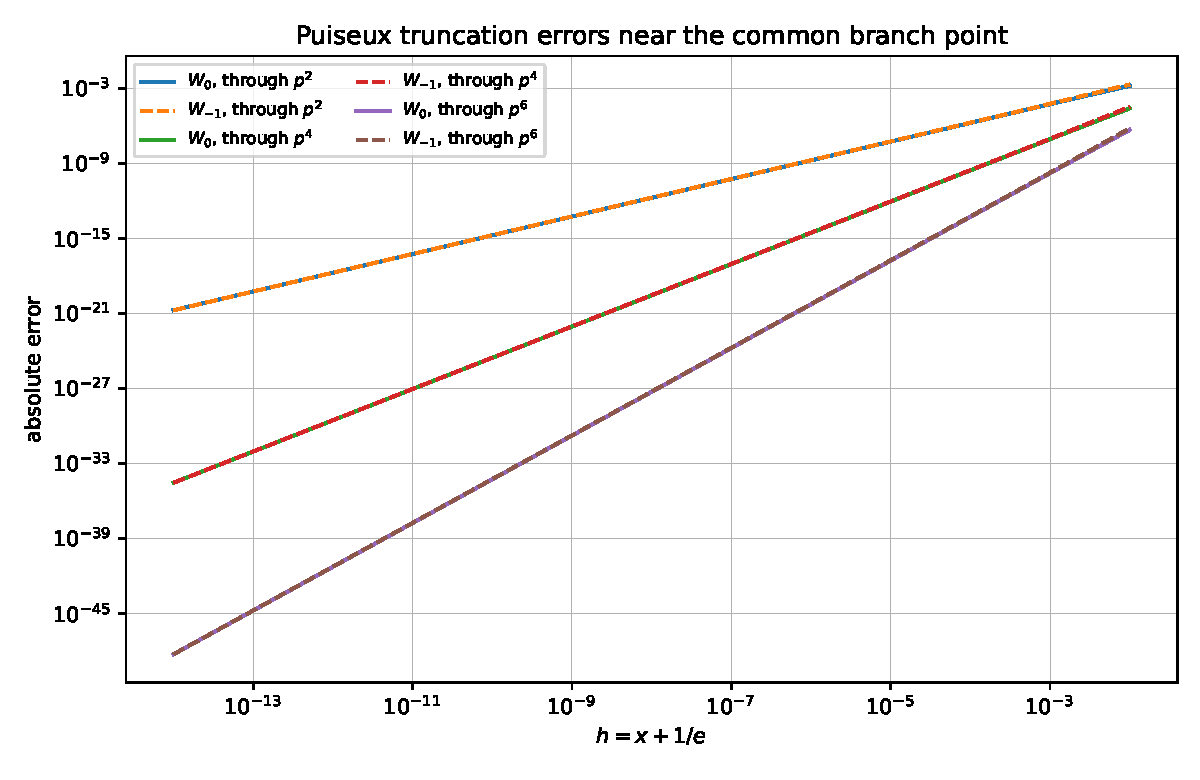
\includegraphics[width=0.9\textwidth]{fig_branch_point_error.pdf}
\caption{Absolute errors of Puiseux truncations on both branches.  Because the
same analytic inverse $U$ controls both branches, their errors have nearly
identical orders.}
\label{fig:branchpointerrors}
\end{figure}

\section{A practical branch-point approximation}

For $x$ close to $-1/\ee$, the variable $p$ is vastly better conditioned than
$x+1/\ee$ itself.  Evaluating \eqref{eq:w0puiseux} or
\eqref{eq:wm1puiseux} through $p^5$ or $p^6$ supplies an excellent initial
value for an iterative method.  It also automatically selects the branch:
use $+p$ for $W_0$ and $-p$ for $W_{-1}$.

Care is needed in floating-point arithmetic when $x$ is supplied as
$-1/\ee+h$ with tiny $h$: computing $1+\ee x$ by naive subtraction may lose
most significant digits.  If $h$ is known separately, compute
$p=\sqrt{2\ee h}$ directly; otherwise use extended precision or a fused
multiply-add operation where available.

\chapter{Logarithmic asymptotic expansions}\label{ch:asymptotics}

\section{Unsigned Stirling numbers of the first kind}

The unsigned Stirling number $\stirlingone{n}{j}$ counts permutations of
$n$ objects with exactly $j$ cycles.  Algebraically it is characterized by
\begin{equation}\label{eq:stirlingrising}
 t(t+1)\cdots(t+n-1)=\sum_{j=0}^{n}\stirlingone{n}{j}t^j.
\end{equation}
We shall use the standard logarithmic coefficient identity
\begin{equation}\label{eq:logstirlingminus}
 [u^n]\bigl(\log(1-u)\bigr)^j
 =(-1)^j\frac{j!}{n!}\stirlingone{n}{j}
 \qquad(n\ge j\ge1).
\end{equation}
It follows by substituting $-u$ into the exponential generating function for
signed Stirling numbers, or by comparing powers in
$(1-u)^t=\exp(t\log(1-u))$.

\section{The principal branch at positive infinity}

Put
\begin{equation}\label{eq:L1L2}
 L_1=\log x,
 \qquad L_2=\log\log x.
\end{equation}
The elementary first approximation is $W_0(x)\approx L_1$, because
$W_0\ee^{W_0}=x$.  Taking a logarithm shows the correction immediately:
$W_0+\log W_0=L_1$, so $W_0\approx L_1-L_2$.

\begin{theorem}[Complete logarithmic expansion of $W_0$]\label{thm:w0asymptotic}
For every fixed $N\ge1$, as $x\to+\infty$,
\begin{align}
 W_0(x)
 &=L_1-L_2
 +\sum_{\ell=1}^{N}\frac1{L_1^\ell}
   \sum_{m=1}^{\ell}
   \frac{(-1)^{\ell-m}}{m!}
   \stirlingone{\ell}{\ell-m+1}L_2^m
 \nonumber\\
 &\quad+\bigO\!\left(\frac{L_2^{N+1}}{L_1^{N+1}}\right).
 \label{eq:w0asymptoticgeneral}
\end{align}
The first terms are
\begin{align}
 W_0(x)={}&L_1-L_2+\frac{L_2}{L_1}
 +\frac{L_2(-2+L_2)}{2L_1^2}
 +\frac{L_2(6-9L_2+2L_2^2)}{6L_1^3}\nonumber\\
 &+\frac{L_2(-12+36L_2-22L_2^2+3L_2^3)}{12L_1^4}\nonumber\\
 &+\frac{L_2(60-300L_2+350L_2^2-125L_2^3+12L_2^4)}{60L_1^5}
 +\cdots.
 \label{eq:w0asymptoticexplicit}
\end{align}
\end{theorem}

\begin{proof}
Write $t=1/L_1$, $B=L_2$, and set
\[
 W_0(x)=L_1(1-y).
\]
The equation $W_0+\log W_0=L_1$ becomes
\begin{equation}\label{eq:yprincipal}
 y=t\bigl(B+\log(1-y)\bigr).
\end{equation}
Treating $B$ as a parameter, Lagrange inversion gives
\[
 y=\sum_{n\ge1}\frac{t^n}{n}
 [u^{n-1}]\bigl(B+\log(1-u)\bigr)^n.
\]
Since $W_0=L_1-y/t$, the coefficient of $t^\ell=L_1^{-\ell}$
for $\ell\ge1$ is
\begin{equation}\label{eq:principalcoefficientproof}
 -\frac1{\ell+1}[u^\ell]
 \bigl(B+\log(1-u)\bigr)^{\ell+1}.
\end{equation}
Expand by the binomial theorem and apply
\eqref{eq:logstirlingminus}.  If $j$ is the power of the logarithm and
$m=\ell+1-j$, expression \eqref{eq:principalcoefficientproof} simplifies to
\[
 \sum_{m=1}^{\ell}
 \frac{(-1)^{\ell-m}}{m!}
 \stirlingone{\ell}{\ell-m+1}B^m,
\]
which proves the coefficient formula.  Finally, $tB=L_2/L_1\to0$.
The analytic implicit-function theorem applied to \eqref{eq:yprincipal}
therefore makes the finite formal expansion asymptotic, with the stated order
of remainder.
\end{proof}

In particular,
\begin{equation}\label{eq:w0twoterm}
 W_0(x)=\log x-\log\log x+o(1).
\end{equation}
The error actually tends to zero, not merely to a bounded quantity.

\section{The lower branch near zero}

For $x\in(-1/\ee,0)$, set
\begin{equation}\label{eq:etaB}
 \eta=\log\frac1{-x}=-\log(-x),
 \qquad B=\log\eta,
 \qquad u=-W_{-1}(x)>1.
\end{equation}
Since $-x=u\ee^{-u}$,
\begin{equation}\label{eq:uminuslogu}
 u-\log u=\eta.
\end{equation}
This is the real lower-branch analogue of $W_0+\log W_0=L_1$.

\begin{theorem}[Complete real expansion of $W_{-1}$]\label{thm:wm1asymptotic}
For every fixed $N\ge1$, as $x\uparrow0$,
\begin{align}
 -W_{-1}(x)
 &=\eta+B
 +\sum_{\ell=1}^{N}\frac1{\eta^\ell}
   \sum_{m=1}^{\ell}
   \frac{(-1)^{m-1}}{m!}
   \stirlingone{\ell}{\ell-m+1}B^m
 \nonumber\\
 &\quad+\bigO\!\left(\frac{B^{N+1}}{\eta^{N+1}}\right).
 \label{eq:wm1asymptoticgeneral}
\end{align}
In particular,
\begin{align}
 W_{-1}(x)=-\Bigg(&\eta+B+\frac{B}{\eta}
 +\frac{B(2-B)}{2\eta^2}
 +\frac{B(6-9B+2B^2)}{6\eta^3}\nonumber\\
 &+\frac{B(12-36B+22B^2-3B^3)}{12\eta^4}\nonumber\\
 &+\frac{B(60-300B+350B^2-125B^3+12B^4)}{60\eta^5}
 +\cdots\Bigg).
 \label{eq:wm1asymptoticexplicit}
\end{align}
\end{theorem}

\begin{proof}
Set $u=\eta(1+y)$ and $t=1/\eta$.  Equation
\eqref{eq:uminuslogu} becomes
\begin{equation}\label{eq:ylower}
 y=t\bigl(B+\log(1+y)\bigr).
\end{equation}
Lagrange inversion yields
\[
 y=\sum_{n\ge1}\frac{t^n}{n}
 [s^{n-1}]\bigl(B+\log(1+s)\bigr)^n.
\]
Now
\[
 [s^\ell]\bigl(\log(1+s)\bigr)^j
 =(-1)^{\ell-j}\frac{j!}{\ell!}
 \stirlingone{\ell}{j}.
\]
Since $u=\eta+y/t$, the same binomial simplification as in the preceding
proof gives the inner sum in \eqref{eq:wm1asymptoticgeneral}.  Because
$B/\eta\to0$, the analytic implicit-function argument again supplies the
remainder estimate.
\end{proof}

The first two terms alone give the memorable rule
\begin{equation}\label{eq:wm1twoterm}
 W_{-1}(x)
 =\log(-x)-\log\bigl(-\log(-x)\bigr)+o(1)
 \qquad(x\uparrow0).
\end{equation}
It looks formally like the $W_0$ expansion, but $\log(-x)$ is large and
negative, so the branch tends to $-\infty$.

\section{Derivatives in the asymptotic regimes}

From \eqref{eq:Wprime},
\begin{align}
 W_0'(x)&=\frac1x\left(1-\frac1{W_0(x)}+\bigO(W_0(x)^{-2})\right)
 &&(x\to\infty),\label{eq:w0primeasymptotic}\\
 W_{-1}'(x)&=\frac1x\left(1-\frac1{W_{-1}(x)}+\bigO(W_{-1}(x)^{-2})\right)
 &&(x\uparrow0).
 \label{eq:wm1primeasymptotic}
\end{align}
The second derivative formula then gives
$W_0''(x)\sim-1/x^2$ and $W_{-1}''(x)\sim-1/x^2$ in their respective limits.
For $W_{-1}$, $x<0$, so $W_{-1}'(x)\sim1/x<0$.

\begin{figure}[htbp]
\centering
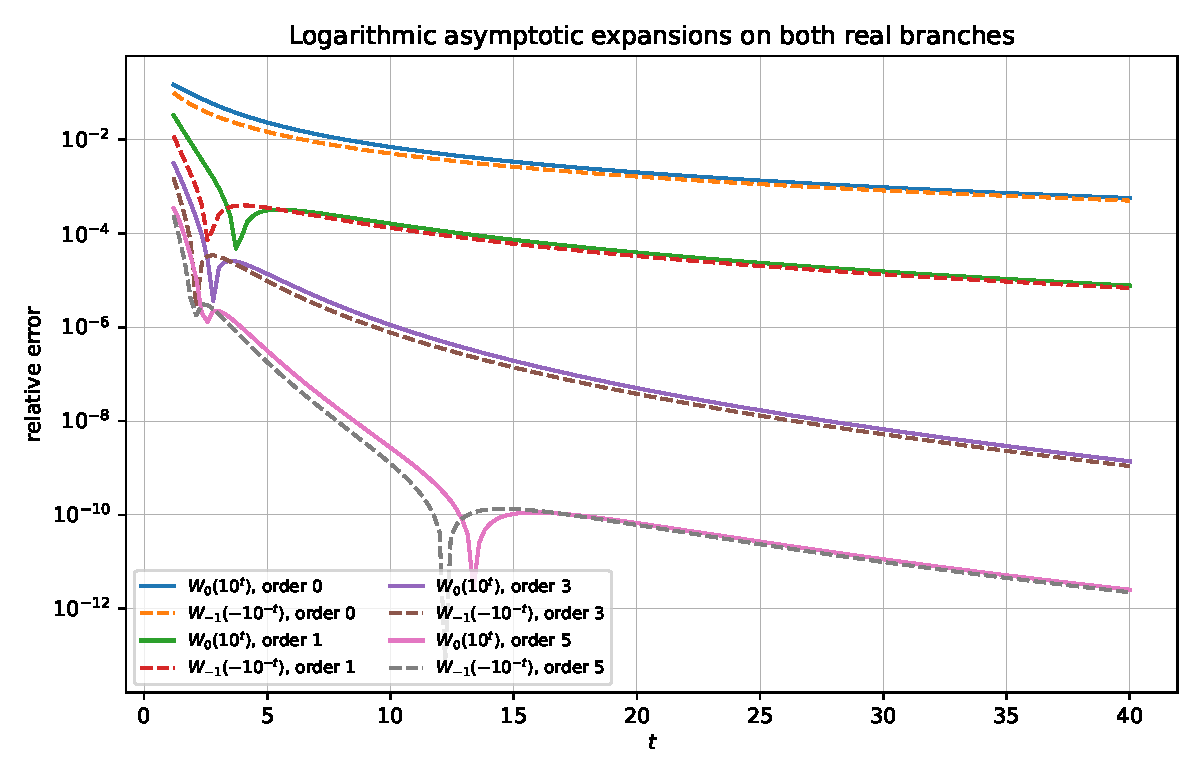
\includegraphics[width=0.9\textwidth]{fig_asymptotic_error.pdf}
\caption{Relative errors of paired logarithmic expansions.  Solid curves use
$W_0(10^t)$; dashed curves use $W_{-1}(-10^{-t})$.  Each additional pair of
terms markedly extends the useful range.}
\label{fig:asymptoticerrors}
\end{figure}

\section{Other complex branches}

Choose a branch of the logarithm and define
\begin{equation}\label{eq:complexL}
 L_{1,k}=\Log z+2\pi\ii k,
 \qquad
 L_{2,k}=\Log L_{1,k}.
\end{equation}
Away from the relevant cuts and Stokes transitions, the same formal expansion
as \eqref{eq:w0asymptoticgeneral} gives
\begin{equation}\label{eq:complexasymptotic}
 W_k(z)\sim L_{1,k}-L_{2,k}
 +\sum_{\ell\ge1}\frac1{L_{1,k}^\ell}
   \sum_{m=1}^{\ell}
   \frac{(-1)^{\ell-m}}{m!}
   \stirlingone{\ell}{\ell-m+1}L_{2,k}^m.
\end{equation}
The integer $k$ enters first through the $2\pi\ii k$ in $L_{1,k}$.  This
explains why the branches are approximately vertically separated by
$2\pi\ii$ for large $|k|$ or large $|z|$.

\chapter{Bounds and inequalities}\label{ch:bounds}

Asymptotic formulas describe limiting behavior, but an inequality gives a
certificate at a finite argument.  This chapter begins with bounds that need
only elementary calculus and then develops sharper estimates adapted to the
lower branch.

\section{Two global bounds for the positive principal branch}

\begin{theorem}\label{thm:w0basicpositivebounds}
For every $x\ge0$,
\begin{equation}\label{eq:w0basicpositivebounds}
 \frac{x}{1+x}\le W_0(x)\le x.
\end{equation}
Both inequalities are strict when $x>0$.
\end{theorem}

\begin{proof}
Put $w=W_0(x)\ge0$, so that $x=w\ee^w$.  Since $\ee^w\ge1$,
$x\ge w$, proving the upper bound.  For the lower bound, after cancelling
$w>0$, the desired inequality is equivalent to
\[
 \frac{\ee^w}{1+w\ee^w}<1,
 \qquad\hbox{or}\qquad
 1+(w-1)\ee^w>0.
\]
The last function is zero at $w=0$ and has derivative $w\ee^w>0$ for
$w>0$.  Hence it is positive there.  At $x=0$ all three quantities in
\eqref{eq:w0basicpositivebounds} vanish.
\end{proof}

For small $x$, the upper bound has the correct leading term.  For large $x$,
logarithmic bounds are much better.

\begin{theorem}[nested-logarithm bounds]\label{thm:nestedlogbounds}
Let $x>\ee$, put $A=\log x$, and define
\begin{equation}\label{eq:nestedlogiterates}
 a_0=A,
 \qquad
 a_{n+1}=A-\log a_n.
\end{equation}
Then every $a_n$ is positive and
\begin{equation}\label{eq:alternatingbounds}
 a_1<a_3<\cdots<W_0(x)<\cdots<a_4<a_2<a_0.
\end{equation}
In particular,
\begin{equation}\label{eq:firstnestedbounds}
 \log x-\log\log x
 <W_0(x)
 <\log x-\log\bigl(\log x-\log\log x\bigr).
\end{equation}
\end{theorem}

\begin{proof}
Write $w=W_0(x)$.  Taking logarithms of $w\ee^w=x$ gives
$w=A-\log w$.  Thus $w$ is a fixed point of the decreasing function
$g(t)=A-\log t$.  Since $A=w+\log w>w>1$, we have $a_0>w$ and hence
$a_1=g(a_0)<g(w)=w$.  Conversely $a_2=g(a_1)>w$.  Also
$A-\log A>1$ for $A>1$, so the whole interval $[a_1,a_0]$ is positive and
is mapped into itself.

The map $g\circ g$ is increasing.  From $a_2<a_0$ it follows inductively
that $a_{2n+2}<a_{2n}$; applying the decreasing map $g$ then shows
$a_{2n+3}>a_{2n+1}$.  The even and odd subsequences are therefore nested
around $w$, proving \eqref{eq:alternatingbounds}.  The first odd and first
nontrivial even bounds give \eqref{eq:firstnestedbounds}.
\end{proof}

The iteration in \eqref{eq:nestedlogiterates} is only linearly convergent,
but its alternation is convenient when a simple symbolic upper and lower
bound is preferable to a high-precision number.

\section{Bounds for $W_0$ on the negative interval}

\begin{theorem}\label{thm:w0negativebounds}
For $-1/\ee<x<0$,
\begin{equation}\label{eq:w0negativebounds}
 -1+\sqrt{1+\ee x}<W_0(x)<x.
\end{equation}
\end{theorem}

\begin{proof}
Let $w=W_0(x)\in(-1,0)$.  Because $\ee^w<1$ and $w<0$,
$x=w\ee^w>w$, which is the upper bound.

For the lower bound put $t=1+w\in(0,1)$.  Since
$x=(t-1)\ee^{t-1}$, the desired inequality is equivalent to
\[
 1+(t-1)\ee^t<t^2.
\]
Define $q(t)=t^2-1-(t-1)\ee^t$.  Then $q(0)=q(1)=0$ and
\[
 q'(t)=t(2-\ee^t).
\]
Thus $q$ increases on $(0,\log2)$ and decreases on $(\log2,1)$.
It is therefore positive throughout $(0,1)$, proving the result.
\end{proof}

The square root in the lower bound is not accidental: it detects the branch
point.  Its coefficient is not optimal---the leading Puiseux term uses
$\sqrt{2(1+\ee x)}$---but the bound remains valid over the entire interval.

\section{Elementary logarithmic bounds for $W_{-1}$}

\begin{theorem}\label{thm:wm1logbounds}
For $-1/\ee\le x<0$,
\begin{equation}\label{eq:wm1logbounds}
 \frac{\ee}{\ee-1}\log(-x)
 \le W_{-1}(x)
 \le \log(-x)-\log\bigl(-\log(-x)\bigr).
\end{equation}
Equality in the right inequality occurs at $x=-1/\ee$; equality in the left
inequality occurs when $W_{-1}(x)=-\ee$.
\end{theorem}

\begin{proof}
Set
\[
 u=-W_{-1}(x)\ge1,
 \qquad
 \eta=-\log(-x)=u-\log u\ge1.
\]
The right inequality in \eqref{eq:wm1logbounds} is equivalent to
$u\ge\eta+\log\eta$.  But $u\ge\eta$ and therefore
$u-\eta=\log u\ge\log\eta$.

For the left inequality, put $c=\ee/(\ee-1)$.  It is equivalent to
$u\le c\eta$.  After multiplying by $\ee-1$, this becomes
\[
 u-\ee\log u\ge0.
\]
The function on the left has derivative $1-\ee/u$, decreases on $[1,\ee]$,
increases on $[\ee,\infty)$, and has minimum zero at $u=\ee$.
\end{proof}

The upper bound is exactly the first two terms of the logarithmic asymptotic
expansion.  The lower bound is coarser near zero, but it is global and has a
short proof.

\section{Square-root bounds for the lower branch}

The following result, adapted from Chatzigeorgiou's analysis
\cite{chatzigeorgiou2013}, is especially useful near $-1/\ee$.

\begin{lemma}\label{lem:logrationalupper}
For $v\ge0$,
\begin{equation}\label{eq:logrationalupper}
 \log(1+v)
 \le v-\frac{v^2}{2(1+v/3)^2}.
\end{equation}
Also $\log(1+v)\ge v-v^2/2$.
\end{lemma}

\begin{proof}
For the first inequality let
\[
 h(v)=\log(1+v)-v+\frac{v^2}{2(1+v/3)^2}.
\]
A direct differentiation gives
\[
 h'(v)=-\frac{v^3(v+9)}{(v+1)(v+3)^3}\le0.
\]
Since $h(0)=0$, we have $h(v)\le0$.  For the second inequality, define
$k(v)=\log(1+v)-v+v^2/2$.  Then
$k'(v)=v^2/(1+v)\ge0$ and $k(0)=0$.
\end{proof}

\begin{theorem}[two-sided branch-point bounds]\label{thm:chatzbounds}
For $s>0$,
\begin{equation}\label{eq:chatzbounds}
 -1-\sqrt{2s}-s
 <W_{-1}\!\left(-\ee^{-1-s}\right)
 <-1-\sqrt{2s}-\frac23s.
\end{equation}
\end{theorem}

\begin{proof}
Write
\[
 W_{-1}(-\ee^{-1-s})=-1-v,
 \qquad v>0.
\]
Substitution into $W\ee^W=-\ee^{-1-s}$ gives
\begin{equation}\label{eq:sgv}
 s=g(v):=v-\log(1+v).
\end{equation}
For a real constant $c$, define
\[
 F_c(v)=c g(v)+\sqrt{2g(v)}-v.
\]
Because $g'(v)=v/(1+v)$,
\begin{equation}\label{eq:Fderivative}
 F_c'(v)=
 \frac{v-\bigl(1+v(1-c)\bigr)\sqrt{2g(v)}}
 {(1+v)\sqrt{2g(v)}}.
\end{equation}
When $c=2/3$, inequality \eqref{eq:logrationalupper} says
$g(v)\ge v^2/[2(1+v/3)^2]$; hence \eqref{eq:Fderivative} is nonpositive.
Since $F_{2/3}(0)=0$, we get
$F_{2/3}(v)<0$ for $v>0$.  When $c=1$, the second part of
\cref{lem:logrationalupper} says $g(v)\le v^2/2$, so
$F_1'(v)\ge0$ and $F_1(v)>0$ for $v>0$.  Therefore
\[
 \frac23s<v-\sqrt{2s}<s.
\]
Equivalently,
$\sqrt{2s}+2s/3<v<\sqrt{2s}+s$.  Replacing $v$ by
$-1-W_{-1}(-\ee^{-1-s})$ reverses the signs and yields
\eqref{eq:chatzbounds}.
\end{proof}

The same parameter $s=-1-\log(-x)$ will provide a guaranteed starting value
for $W_{-1}$ in Chapter~\ref{ch:numerics}.

\section{Transporting bounds through monotone functions}

A bound on $W$ immediately produces many others.  For example,
$\ee^{W_0(x)}=x/W_0(x)$, so positive lower and upper bounds
$L(x)<W_0(x)<U(x)$ give
\[
 \frac{x}{U(x)}<\ee^{W_0(x)}<\frac{x}{L(x)}.
\]
If a solution is $y=A+B W_k(C)$, the order is preserved when $B>0$ and
reversed when $B<0$.  This elementary observation is valuable in applications:
one should propagate the inequality only after checking both the branch and
the sign of every prefactor.


\chapter{Integral, contour, and continued-fraction representations}
\label{ch:representations}

A representation is useful when it exposes structure that the defining
implicit equation hides.  Some representations are naturally principal-branch
objects; the failure to extend them to $W_{-1}$ is itself informative.

\section{The Wright omega function}

For real $t$, define the Wright omega function by
\begin{equation}\label{eq:wrightomega}
 \omega(t)=W_0(\ee^t).
\end{equation}
It is the unique positive solution of
\begin{equation}\label{eq:omegaequation}
 \omega+\log\omega=t.
\end{equation}
Conversely, $W_0(x)=\omega(\log x)$ for $x>0$.  Differentiation gives
\begin{equation}\label{eq:omegaderivative}
 \omega'(t)=\frac{\omega(t)}{1+\omega(t)}.
\end{equation}
This form avoids constructing the possibly enormous number $\ee^t$ and is
therefore often preferable in floating-point computation.  In the complex
plane the standard Wright omega function incorporates an ``unwinding
number'' that selects the appropriate logarithm; see Corless and Jeffrey for
the full branch convention.

For the lower real branch it is more natural to use
$u=-W_{-1}(-\ee^{-\eta})$, which satisfies
$u-\log u=\eta$.  The change of sign in front of the logarithm is precisely
what distinguishes the lower-branch asymptotic expansion from
\eqref{eq:omegaequation}.

\section{A contour formula for any simple branch value}

\begin{theorem}\label{thm:contourW}
Let $z\in\C$, and let $\Gamma$ be a positively oriented simple closed contour
in the $w$-plane.  Suppose $w\ee^w-z$ has exactly one zero $w_k$ inside
$\Gamma$, that zero is simple, and there are no zeros on $\Gamma$.  Then
\begin{equation}\label{eq:contourW}
 w_k=\frac{1}{2\pi\ii}
 \int_\Gamma
 \frac{w\,\ee^w(1+w)}{w\ee^w-z}\,dw.
\end{equation}
Thus, when the contour isolates the $k$th inverse value, the right side equals
$W_k(z)$.
\end{theorem}

\begin{proof}
The integrand is $w f'(w)/(f(w)-z)$ with $f(w)=w\ee^w$.  At a simple zero
$w_k$, its residue is
\[
 \frac{w_k f'(w_k)}{f'(w_k)}=w_k.
\]
There are no other poles inside $\Gamma$, so the residue theorem gives
\eqref{eq:contourW}.
\end{proof}

At $z=-1/\ee$ the zero $w=-1$ is double because $f'(-1)=0$; the hypotheses
then fail.  This is the contour-theoretic reflection of the square-root branch
point.

\section{A Fourier--logarithm integral for $W_0$}

The following representation is a transparent consequence of the Taylor
series and Fourier orthogonality.  Corcino, Corcino, and Mezo extend the same
integral, with a careful continuous choice of logarithm, to the real interval
$[-1/\ee,\ee]$ \cite{corcino2018}.

\begin{theorem}\label{thm:fourierlogintegral}
For real $|x|<1/\ee$,
\begin{equation}\label{eq:fourierlogintegral}
 W_0(x)=\frac1\pi\operatorname{Re}\int_0^\pi
 \log\!\left(
 \frac{\exp(\ee^{\ii t})-x\ee^{-\ii t}}
      {\exp(\ee^{\ii t})-x\ee^{\ii t}}
 \right)dt,
\end{equation}
where the logarithm is obtained by its power series at $x=0$.
\end{theorem}

\begin{proof}
Let $A(t)=\exp(\ee^{\ii t})$.  Since
$|x\ee^{\pm\ii t}/A(t)|\le \ee|x|<1$, both logarithms may be expanded
uniformly and integrated term by term.  Their difference is
\begin{align*}
 \log\frac{A-x\ee^{-\ii t}}{A-x\ee^{\ii t}}
 &=2\ii\sum_{n\ge1}\frac{x^n}{n}
      \ee^{-n\ee^{\ii t}}\sin(nt).
\end{align*}
Expand once more:
\[
 \ee^{-n\ee^{\ii t}}
 =\sum_{j\ge0}\frac{(-n)^j}{j!}\ee^{\ii jt}.
\]
Because $\operatorname{Re}(\ii\ee^{\ii jt})=-\sin(jt)$ and
\[
 \int_0^\pi\sin(jt)\sin(nt)\,dt=
 \begin{cases}\pi/2,&j=n,\\0,&j\ne n,\end{cases}
\]
the coefficient of $x^n$ on the right of
\eqref{eq:fourierlogintegral} is
\[
 -\frac{(-n)^n}{n\,n!}=\frac{(-n)^{n-1}}{n!}.
\]
These are exactly the Taylor coefficients in
\eqref{eq:Wseries}, proving the identity.
\end{proof}

There is no analogous Taylor-based integral centered at zero for $W_{-1}$:
that branch diverges logarithmically as $x\uparrow0$.  A lower-branch integral
must instead be based on a branch-point or logarithmic coordinate.

\section{Euler's conversion of a series to a continued fraction}

\begin{lemma}[Euler's finite identity]\label{lem:eulercf}
Let $c_1,\ldots,c_N$ be nonzero and put $r_m=c_{m+1}/c_m$.  Then
\begin{equation}\label{eq:eulercffinite}
 \sum_{m=1}^N c_m
 =\cfrac{c_1}{1+
   \cfrac{-r_1}{1+r_1+
   \cfrac{-r_2}{1+r_2+
   \cfrac{\ddots}{\ddots+
   \cfrac{-r_{N-1}}{1+r_{N-1}}}}}}.
\end{equation}
\end{lemma}

\begin{proof}
Write $R_m=c_m+\cdots+c_N$.  Starting from the bottom, one verifies by
backward induction that the tail denominator beginning with $1+r_m$ equals
$r_mR_m/R_{m+1}$.  Consequently the entire denominator in
\eqref{eq:eulercffinite} is
$1-R_2/R_1=c_1/R_1$, and the fraction equals $R_1$.
\end{proof}

Apply this identity to
$c_n=(-n)^{n-1}x^n/n!$.  A calculation gives
\[
 \frac{c_{m+1}}{c_m}=-\rho_m x,
 \qquad
 \rho_m=\left(1+\frac1m\right)^{m-1}.
\]
Taking the limit of the finite identities therefore yields the following
continued fraction wherever the Taylor series converges and no finite
denominator vanishes:
\begin{equation}\label{eq:eulerWcf}
 W_0(x)=
 \cfrac{x}{1+
  \cfrac{\rho_1x}{1-\rho_1x+
  \cfrac{\rho_2x}{1-\rho_2x+
  \cfrac{\rho_3x}{1-\rho_3x+\ddots}}}}.
\end{equation}
Interpreted as the limit of its finite truncations, this is simply a
repackaging of the convergent Taylor series for $|x|<1/\ee$.

Corcino, Corcino, and Mezo also derive a regular C-fraction beginning
\begin{equation}\label{eq:corcinocf}
 W_0(x)=\cfrac{x}{1+
 \cfrac{x}{1+
 \cfrac{x/2}{1+
 \cfrac{5x/6}{1+
 \cfrac{17x/30}{1+\ddots}}}}},
\end{equation}
with general coefficients expressed through Hankel determinants and computable
by the quotient--difference algorithm \cite{corcino2018}.  Continued
fractions can outperform a raw Taylor polynomial near a boundary of
convergence, but their poles must be monitored.  Again, a fraction derived
from analyticity at zero represents $W_0$, not $W_{-1}$.

\section{Inverse-function integrals and moments}

The substitution $x=w\ee^w$ from Chapter~\ref{ch:integrals} may itself be
viewed as an integral representation.  For any continuous $F$ and any real
branch segment on which the endpoints correspond to $w=a$ and $w=b$,
\begin{equation}\label{eq:momentrepresentation}
 \int_{a\ee^a}^{b\ee^b}F(W_k(x))\,dx
 =\int_a^b F(w)\ee^w(1+w)\,dw.
\end{equation}
The branch is encoded by the allowed $w$-interval: $[-1,\infty)$ for $W_0$
and $(-\infty,-1]$ for $W_{-1}$.  Formula
\eqref{eq:momentrepresentation} is often a simpler representation than any
integral whose integrand still contains $W$.


\chapter{Reliable numerical evaluation and practical approximations}
\label{ch:numerics}

No single truncated formula is uniformly excellent on an entire real branch.
A reliable implementation therefore combines three ideas:
\begin{enumerate}
\item choose a local coordinate suited to the region;
\item choose the branch before iterating;
\item finish with a rapidly convergent correction whose iterates cannot jump
to the other real branch.
\end{enumerate}
The source archive contains several generations of this strategy, from the
analytic approximations of Barry and coauthors \cite{barry2000}, through the
global principal-branch approximation of Iacono and Boyd
\cite{iacono2017}, to the guaranteed high-precision analysis of Loczi
\cite{loczi2022} and the high-order Schroder expansions of Howard
\cite{howard2025}.

\section{Newton and Halley applied directly}

For
\[
 f_x(w)=w\ee^w-x,
 \qquad
 f_x'(w)=\ee^w(1+w),
 \qquad
 f_x''(w)=\ee^w(2+w),
\]
Newton's method is
\begin{equation}\label{eq:directnewton}
 w_{n+1}
 =w_n-\frac{w_n\ee^{w_n}-x}{\ee^{w_n}(1+w_n)}
 =w_n-\frac{w_n-x\ee^{-w_n}}{1+w_n}.
\end{equation}
The second form avoids one exponential in the numerator, but it can still
overflow or underflow when $x$ and $w_n$ are extreme.

Halley's method is
\begin{equation}\label{eq:halley}
 w_{n+1}=w_n-
 \frac{w_n\ee^{w_n}-x}
 {\ee^{w_n}(1+w_n)-
 \dfrac{(w_n+2)(w_n\ee^{w_n}-x)}{2(1+w_n)}}.
\end{equation}
At a simple root, Newton is locally quadratic and Halley is locally cubic.

\begin{proposition}\label{prop:newtonhalleyorders}
Let $f$ have three continuous derivatives near a simple zero $r$.
For starts sufficiently near $r$, Newton's errors satisfy
$e_{n+1}=\bigl(f''(r)/(2f'(r))\bigr)e_n^2+\bigO(e_n^3)$, while Halley's
errors are $\bigO(e_n^3)$.
\end{proposition}

\begin{proof}
Write $y=r+e$ and expand
\[
 f(y)=a e+\frac b2e^2+\frac c6e^3+\bigO(e^4),
 \qquad
 f'(y)=a+b e+\frac c2e^2+\bigO(e^3),
\]
where $a=f'(r)\ne0$.  Division of the two series gives
$f(y)/f'(y)=e-(b/2a)e^2+\bigO(e^3)$, which proves the Newton formula.
For Halley, substitute the same expansions into
$y-2ff'/(2(f')^2-ff'')$; the coefficients of $e$ and $e^2$ cancel, leaving
an error of order $e^3$.
\end{proof}

The qualifier ``simple'' matters.  At $x=-1/\ee$, the root $w=-1$ is double,
$f_x'(-1)=0$, and both displayed formulas have a singular denominator.
Near that point the Puiseux coordinate is the right starting language.

\section{A logarithmic Newton map}

For real $x$ and a real iterate $b$ of the same sign, the equation
$b\ee^b=x$ is equivalent to
\begin{equation}\label{eq:logrootfunction}
 F_x(b):=b+\log|b|-\log|x|=0.
\end{equation}
Newton's method for $F_x$ is
\begin{equation}\label{eq:lognewton}
 \boxed{\quad
 T_x(b)=\frac{b}{1+b}\left(1+\log\frac{x}{b}\right).
 \quad}
\end{equation}
The ratio $x/b$ is positive, so the logarithm is real on both real branches.
This iteration was emphasized by Iacono and Boyd and analyzed globally with
explicit error bounds by Loczi \cite{iacono2017,loczi2022}.  It needs no
exponential and is well scaled for $W_0(x)$ at huge positive $x$ and for
$W_{-1}(x)$ at tiny negative $x$.

The following theorem gives a self-contained branch-safe convergence result.

\begin{theorem}[three monotone invariant intervals]
\label{thm:lognewtonmonotone}
Let $w$ be the indicated real solution of $w\ee^w=x$.
\begin{enumerate}[label=(\alph*)]
\item If $w>0$ and $0<b_0<w$, then
$0<b_0<b_1<\cdots<w$, and $b_n\to w$.
\item If $-1<w<0$ and $w<b_0<0$, then
$w<\cdots<b_2<b_1<b_0<0$, and $b_n\to w$.
\item If $w<-1$ and $b_0<w$, then
$b_0<b_1<b_2<\cdots<w$, and $b_n\to w$.
\end{enumerate}
Here $b_{n+1}=T_x(b_n)$.
\end{theorem}

\begin{proof}
For any admissible $b$, put $r=b/w>0$.  Since
$x=w\ee^w$, direct simplification gives the two exact identities
\begin{align}
 T_x(b)-w
 &=\frac{w\bigl(r-1-r\log r\bigr)}{1+b},
 \label{eq:Texactrootdifference}\\
 T_x(b)-b
 &=\frac{b}{1+b}\left(\log\frac wb+w-b\right).
 \label{eq:Texactstepdifference}
\end{align}
The function $h(r)=r-1-r\log r$ has derivative $-\log r$ and unique maximum
$h(1)=0$.  Thus $h(r)<0$ when $r\ne1$.

In case (a), $0<r<1$.  Equation
\eqref{eq:Texactrootdifference} gives $T_x(b)<w$, while both terms in the
parentheses of \eqref{eq:Texactstepdifference} are positive, so $T_x(b)>b$.

In case (b), again $0<r<1$.  Now $w<0$ and $1+b>0$, so
\eqref{eq:Texactrootdifference} gives $T_x(b)>w$.  Moreover
\[
 \log\frac wb+w-b=-\log r+w(1-r)> (1-r)-(1-r)=0,
\]
because $-\log r>1-r$ and $w>-1$.  Since $b/(1+b)<0$,
\eqref{eq:Texactstepdifference} gives $T_x(b)<b$.

In case (c), $r>1$, $w<0$, and $1+b<0$, so
\eqref{eq:Texactrootdifference} gives $T_x(b)<w$.  Also
\[
 \log\frac wb+w-b=-\log r+(-w)(r-1)>-\log r+r-1>0.
\]
Here $b/(1+b)>0$, hence $T_x(b)>b$.

Each sequence is monotone and bounded, so it has a limit $\ell$.  Passing to
the limit in \eqref{eq:lognewton} gives
$\log(x/\ell)=\ell$, hence $\ell\ee^\ell=x$.  The invariant interval contains
only the specified real root, so $\ell=w$.
\end{proof}

\begin{corollary}[quadratic error constant]\label{cor:lognewtonquadratic}
For $b=w+e$ near a real root $w\ne-1,0$,
\begin{equation}\label{eq:lognewtonerror}
 T_x(b)-w
 =-\frac{e^2}{2w(1+w)}+\bigO(e^3).
\end{equation}
Thus the convergence in \cref{thm:lognewtonmonotone} is quadratic once the
iterates are near the root.
\end{corollary}

\begin{proof}
Set $r=1+e/w$ in \eqref{eq:Texactrootdifference} and use
\[
 r-1-r\log r=-\frac12(r-1)^2+\frac16(r-1)^3+\bigO((r-1)^4).
\]
Expanding $1/(1+w+e)$ gives \eqref{eq:lognewtonerror}.
\end{proof}

\section{Explicit global starting values}

\begin{algorithm}[branch-safe real starts]\label{alg:realstarts}
Handle $x=-1/\ee$, $x=0$, and $x=\ee$ exactly.  Otherwise use
\begin{align}
 b_0&=x,
 &&-1/\ee<x<0,\quad W_0,\label{eq:startw0neg}\\
 b_0&=x/\ee,
 &&0<x<\ee,\quad W_0,\label{eq:startw0smallpos}\\
 b_0&=\log x-\log\log x,
 &&x>\ee,\quad W_0,\label{eq:startw0large}\\
 b_0&=-1-\sqrt{2s}-s,
 \quad s=-1-\log(-x),
 &&-1/\ee<x<0,\quad W_{-1}.
 \label{eq:startwm1}
\end{align}
Then iterate \eqref{eq:lognewton}.
\end{algorithm}

\begin{theorem}\label{thm:startsvalid}
Every start in \cref{alg:realstarts} satisfies the corresponding hypothesis
of \cref{thm:lognewtonmonotone}; consequently it converges monotonically to
the requested branch value.
\end{theorem}

\begin{proof}
For \eqref{eq:startw0neg}, if $w=W_0(x)\in(-1,0)$ then
$x=w\ee^w>w$, so $w<x<0$.  For \eqref{eq:startw0smallpos}, $W_0$ is strictly
concave on $(0,\infty)$, and the chord joining $(0,0)$ and $(\ee,1)$ is
$x/\ee$; hence $0<x/\ee<W_0(x)$ for $0<x<\ee$.

For \eqref{eq:startw0large}, put $A=\log x>1$ and
$b_0=A-\log A>1$.  Since
$b_0\ee^{b_0}=x b_0/A<x$ and $w\mapsto w\ee^w$ is increasing for $w>-1$,
we have $b_0<W_0(x)$.

Finally \eqref{eq:startwm1} is precisely the strict lower bound in
\eqref{eq:chatzbounds}.  The three cases now follow from
\cref{thm:lognewtonmonotone}.
\end{proof}

The starts are deliberately simple rather than minimax-optimal.  Loczi gives
piecewise starts with explicit uniform errors that square at every step;
Howard constructs generic Schroder series from an initial approximating
function and reports extremely high accuracy at high order
\cite{loczi2022,howard2025}.

\section{A posteriori error certification}

An iterate should be stopped because its error is bounded, not merely because
successive floating-point numbers happen to be equal.

\begin{proposition}\label{prop:residualbound}
Let $I$ be an interval containing a unique root $w$ of $F_x$ in
\eqref{eq:logrootfunction}.  If
$|F_x'(t)|\ge m>0$ throughout $I$, then every $b\in I$ satisfies
\begin{equation}\label{eq:residualbound}
 |b-w|\le\frac{|F_x(b)|}{m},
 \qquad
 F_x'(t)=1+\frac1t.
\end{equation}
\end{proposition}

\begin{proof}
The mean-value theorem gives
$F_x(b)-F_x(w)=F_x'(\xi)(b-w)$ for some $\xi$ between $b$ and $w$.
Take absolute values and use $F_x(w)=0$.
\end{proof}

For $W_0(x)>0$, one may take the crude universal value $m=1$.  On either
negative branch, $|1+1/t|$ tends to zero as $t\to-1$, so no residual bound in
the original $w$ coordinate can remain uniform at the branch point.  There,
the $p$ coordinate of Chapter~\ref{ch:branchpoint} supplies the appropriate
conditioning.

A robust implementation can maintain a one-sided monotone bound from
\cref{thm:lognewtonmonotone}, compute a second bound from an analytic
inequality, and then stop when the bracket width is below the requested
tolerance.  For ordinary machine precision, the combination of a region-aware
start and two or three Halley or logarithmic-Newton corrections is generally
more than sufficient.

\begin{figure}[htbp]
\centering
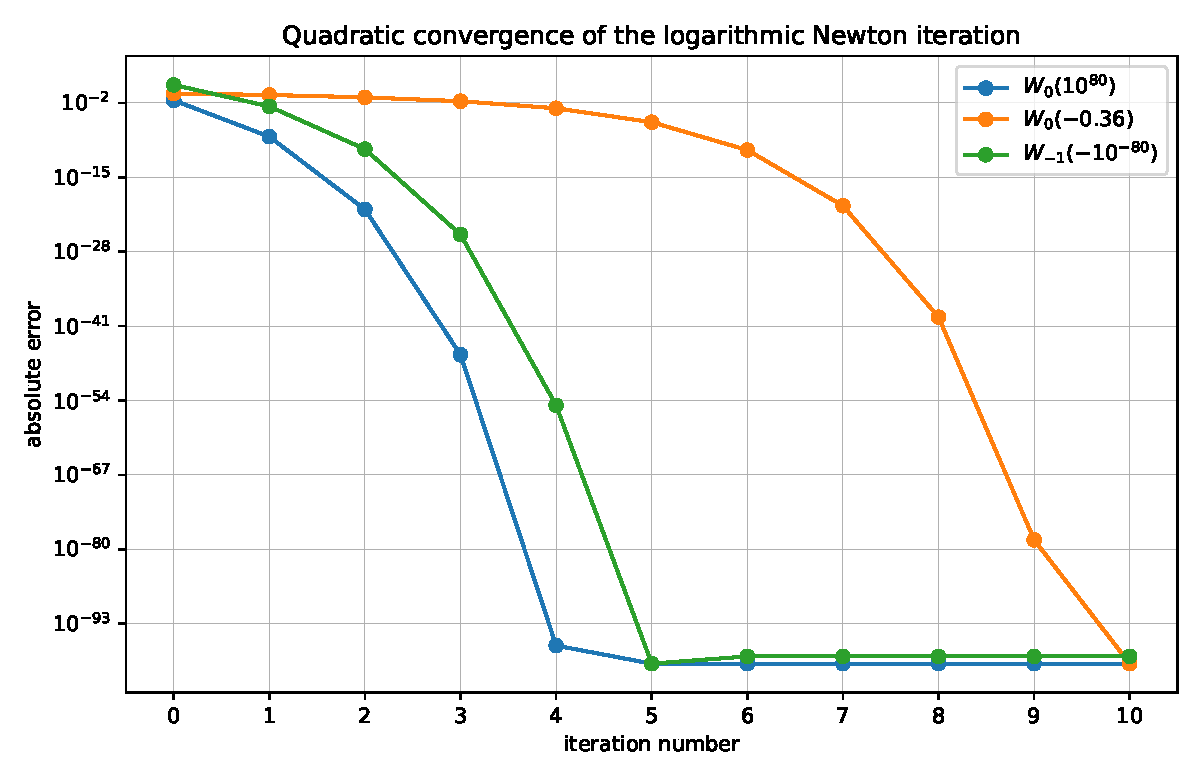
\includegraphics[width=0.9\textwidth]{fig_iteration_error.pdf}
\caption{Absolute error under the logarithmic Newton iteration for a huge
positive argument, a point close to the branch point on $W_0$, and a tiny
negative argument on $W_{-1}$.  The slopes steepen in accordance with
quadratic convergence until the working precision is reached.}
\label{fig:iterationerrors}
\end{figure}

\section{Choosing an approximation by region}

\begin{center}
\begin{tabular}{@{}p{0.19\textwidth}p{0.23\textwidth}p{0.23\textwidth}p{0.24\textwidth}@{}}
\toprule
Region & Natural coordinate & Good first approximation & Main caution\\
\midrule
$W_0$, $|x|\ll1$ & $x$ & Taylor series
\eqref{eq:Wseries} & radius is exactly $1/\ee$\\
Either branch near $-1/\ee$ & $p=\sqrt{2(1+\ee x)}$ & paired Puiseux series
\eqref{eq:w0puiseux}, \eqref{eq:wm1puiseux} & subtraction in $1+\ee x$\\
$W_0$, $x\gg1$ & $(\log x,\log\log x)$ &
\eqref{eq:w0asymptoticexplicit} & asymptotic, not a small-$x$ series\\
$W_{-1}$, $x\uparrow0$ &
$\eta=\log(1/(-x))$ & \eqref{eq:wm1asymptoticexplicit} & preserve the lower
branch and the sign\\
Middle of a branch & $w$ itself & monotone start plus
\eqref{eq:lognewton} & never cross $w=-1$\\
\bottomrule
\end{tabular}
\end{center}

A practical composite evaluator is therefore:
\begin{enumerate}
\item use a Puiseux truncation when $1+\ee x$ is small;
\item otherwise use a Taylor or logarithmic truncation when its natural
small parameter is small;
\item otherwise use \cref{alg:realstarts};
\item apply logarithmic Newton or Halley until a residual or bracket test
passes.
\end{enumerate}
The accompanying program implements and tests these ingredients.  It uses
high-precision reference values only to produce the figures; the formulas
being tested are coded explicitly.

\section{Published global approximations in the archive}

It is useful to distinguish an \emph{analytic approximation}, intended to be
inserted into further algebra, from a \emph{numerical seed}, intended only to
start an iteration.

Barry, Parlange, Li, Prommer, Cunningham, and Stagnitti construct separate
closed forms for the three real pieces $W_{-1}$, $W_0|_{[-1/\ee,0]}$, and
$W_0|_{[0,\infty)}$, arranging exact endpoint behavior and small reported
maximum relative errors \cite{barry2000}.  This separation is mathematically
natural: no expression analytic at zero can simultaneously represent the
unbounded branch $W_{-1}$.

Iacono and Boyd give a simple global approximation to $W_0$ with reported
maximum relative error below $5\times10^{-3}$, then reach machine precision
with three steps of the logarithmic Newton map
\eqref{eq:lognewton}; they also derive tight large-$x$ bounds and discuss
Chebyshev approximations \cite{iacono2017}.  Chebyshev polynomials work best
after a change of variable that resolves both the square-root singularity at
$-1/\ee$ and the logarithmic growth at infinity.

Howard's Schroder-type construction starts with an arbitrary approximating
function lying inside proved upper and lower envelopes and generates an
inverse-function series of arbitrary order for either real branch
\cite{howard2025}.  It provides a systematic bridge between a compact
closed-form seed and very high precision.  The conceptual lesson is broader
than any one formula: a good coordinate and a certified basin are more
important than a long polynomial in the original variable.

\section{Floating-point hazards}

\begin{enumerate}
\item Near $-1/\ee$, the expression $1+\ee x$ loses relative accuracy by
cancellation.  If the input is naturally $x=-1/\ee+h$, compute $p$ from $h$;
otherwise use a fused multiply--add when available.
\item Near $x=0^-$ on $W_{-1}$, forming $x$ may underflow even though
$\log(-x)$ is representable.  An interface accepting $\log(-x)$ directly is
more robust.
\item In \eqref{eq:lognewton}, evaluate $\log(x/b)$ as
$\log|x|-\log|b|$ when the ratio would overflow or underflow.
\item Relative error in $W_0(x)$ is ill-conditioned at $x=0$, where the true
value vanishes.  Use absolute error there.
\item A tiny residual $w\ee^w-x$ does not by itself guarantee a tiny error
near the double root at $-1/\ee$; account for the small derivative or use the
Puiseux coordinate.
\end{enumerate}


\chapter{Complex branches and analytic structure}\label{ch:complex}

The two real graphs are only boundary traces of a countable family of complex
inverse branches.  This chapter gives the minimum complex analysis needed to
understand where those branches come from and why the real singularities have
the forms already derived.

\section{Critical and asymptotic values of $w\ee^w$}

Let $f(w)=w\ee^w$.  It is entire and
\[
 f'(w)=\ee^w(1+w).
\]
Thus its only finite critical point is $w=-1$, and the corresponding critical
value is $-1/\ee$.  The local expansion
\[
 f(-1+u)=-\frac1\ee+\frac{u^2}{2\ee}+\frac{u^3}{3\ee}+\cdots
\]
starts with $u^2$; locally, inversion must therefore introduce a square root.
This recovers the Puiseux behavior of Chapter~\ref{ch:branchpoint} without any
real-variable graph.

There is also an inverse singularity over $z=0$.  Although $f(0)=0$ gives the
regular principal value $W_0(0)=0$, one has $w\ee^w\to0$ along paths with
$\operatorname{Re}w\to-\infty$.  The nonprincipal inverse branches therefore
run off to infinity as $z\to0$, producing logarithmic branch points.

\section{Standard branch domains}

The analytic inverse-function theorem gives a local holomorphic inverse at
every point where $w\ne-1$.  Global single-valued branches require cuts.
Under the standard convention used by Corless et al. and the DLMF
\cite{corless1996,dlmf413}:
\begin{itemize}
\item $W_0$ is analytic on $\C\setminus(-\infty,-1/\ee]$ and is real on
$(-1/\ee,\infty)$;
\item the nonprincipal branches $W_k$, $k\ne0$, are represented on cut planes
with a cut ending at $0$; they have logarithmic behavior there;
\item the sheets adjacent to $W_0$ meet it at the square-root point
$-1/\ee$.  The real function $W_{-1}$ is the lower real boundary value on
$(-1/\ee,0)$.
\end{itemize}
Different software systems may place boundary values on different lips of a
cut.  An index $k$ is therefore meaningful only together with a stated
logarithm convention.

\section{Why there are infinitely many branches}

Taking a logarithm of $w\ee^w=z$ gives, formally,
\begin{equation}\label{eq:complexbranchequation}
 w+\Log w=\Log z+2\pi\ii n,
 \qquad n\in\Z.
\end{equation}
For large $|n|$, the right side has imaginary part approximately $2\pi n$,
and a solution exists near it.  The asymptotic expansion
\eqref{eq:complexasymptotic} makes this precise.  In particular,
\begin{equation}\label{eq:branchspacing}
 W_{k+1}(z)-W_k(z)=2\pi\ii+\bigO\!\left(\frac1k\right)
 \qquad(|k|\to\infty),
\end{equation}
for fixed nonzero $z$ away from cuts.

A circuit around $z=0$ changes $\Log z$ by $2\pi\ii$.  Equation
\eqref{eq:complexbranchequation} then moves the analytic continuation to a
neighboring sheet.  This phenomenon is called \emph{monodromy}; the branch
index records how many logarithmic turns have been made.

\section{Local behavior at zero on nonprincipal branches}

Let
\[
 L_{1,k}=\Log z+2\pi\ii k,
 \qquad L_{2,k}=\Log L_{1,k}.
\]
Then, as $z\to0$ along a fixed sector on a nonprincipal sheet,
\begin{equation}\label{eq:nonprincipalzero}
 W_k(z)=L_{1,k}-L_{2,k}
 +\frac{L_{2,k}}{L_{1,k}}
 +\bigO\!\left(\frac{L_{2,k}^2}{L_{1,k}^2}\right).
\end{equation}
This is the same logarithmic inversion mechanism as at large $z$; what matters
is that $|L_{1,k}|$ is large.  The real lower-branch formula
\eqref{eq:wm1twoterm} is the cut-boundary version of this statement, rewritten
with entirely real logarithms.

\section{Conjugation and real coefficients}

Because $f(\overline w)=\overline{f(w)}$, complex solutions occur in conjugate
pairs.  On any conjugation-symmetric region avoiding the cuts, branch labels
can be chosen so that
\begin{equation}\label{eq:conjugation}
 \overline{W_k(z)}=W_{-k}(\overline z).
\end{equation}
For the principal branch this reduces to
$\overline{W_0(z)}=W_0(\overline z)$.  On a cut one must specify upper and
lower boundary values; conjugation interchanges the two lips.

\section{A transcendence consequence}

\begin{theorem}\label{thm:transcendence}
If $z\ne0$ is algebraic, then every value $W_k(z)$ is transcendental.
\end{theorem}

\begin{proof}
Suppose $w=W_k(z)$ were algebraic.  It is nonzero because $z\ne0$.
The Lindemann--Weierstrass theorem says that $\ee^w$ is transcendental for
nonzero algebraic $w$.  But $w\ee^w=z$ gives
$\ee^w=z/w$, which would be algebraic.  This contradiction proves the claim.
\end{proof}

Thus even the omega constant $W_0(1)$ is transcendental.  The theorem does not
say that values at transcendental arguments must be transcendental; special
cancellations can occur, as the next chapter shows.


\chapter{Identities, branch exchange, and special values}
\label{ch:identities}

Many attractive Lambert identities are really statements of the form
``these two expressions have the same product with their exponential.''  The
last step must always specify which inverse branch returns the proposed value.

\section{Values generated from a chosen output}

For every complex $a$,
\begin{equation}\label{eq:manufacturedvalue}
 W_k(a\ee^a)=a
\end{equation}
whenever the $k$th branch is the inverse sheet containing $a$.  On the real
axis this specializes to
\begin{align}
 W_0(a\ee^a)&=a &&(a\ge-1),\label{eq:manufacturedw0}\\
 W_{-1}(a\ee^a)&=a &&(a\le-1).\label{eq:manufacturedwm1}
\end{align}
This is the safest way to manufacture exact values.  Examples are
\begin{align*}
 W_0(0)&=0,&
 W_0(\ee)&=1,&
 W_0(-1/\ee)&=W_{-1}(-1/\ee)=-1,\\
 W_{-1}(-2\ee^{-2})&=-2,&
 W_{-1}(-3\ee^{-3})&=-3.&
\end{align*}
The principal value $\Omega=W_0(1)$ is the unique positive solution of
$\Omega\ee^\Omega=1$, equivalently $\Omega=\ee^{-\Omega}$.

A complex example is
\begin{equation}\label{eq:complexspecial}
 \left(\frac{\pi\ii}{2}\right)
 \exp\!\left(\frac{\pi\ii}{2}\right)=-\frac\pi2.
\end{equation}
Thus $\pi\ii/2$ and $-\pi\ii/2$ are conjugate Lambert values of $-\pi/2$ on
the two sides of the principal cut.

\section{The real branch-exchange involution}

The function $q\mapsto q\ee^{-q}$ increases on $(0,1]$ and decreases on
$[1,\infty)$.  Therefore every $0<y<1/\ee$ has two positive preimages, one on
each side of $1$.

\begin{definition}
For $0<t\le1$, define
\begin{equation}\label{eq:branchinvolution}
 \sigma(t)=-W_{-1}(-t\ee^{-t}).
\end{equation}
Then $\sigma(t)\ge1$ and
$t\ee^{-t}=\sigma(t)\ee^{-\sigma(t)}$.
\end{definition}

Conversely, for $s\ge1$,
\begin{equation}\label{eq:branchinvolutioninverse}
 -W_0(-s\ee^{-s})\in(0,1]
\end{equation}
returns the partner on the other side.  These operations are inverses.  They
make explicit that $W_0$ and $W_{-1}$ are not unrelated functions: on the
negative real interval they encode the two inverse sides of the same unimodal
map.

\section{An addition identity with a branch condition}

\begin{proposition}\label{prop:additionidentity}
Let $a=W_j(x)$ and $b=W_k(y)$ be nonzero.  Then
\begin{equation}\label{eq:additionidentity}
 (a+b)\ee^{a+b}
 =xy\left(\frac1a+\frac1b\right).
\end{equation}
Consequently,
\begin{equation}\label{eq:additionW}
 a+b=W_\ell\!\left(
 xy\left(\frac1a+\frac1b\right)\right)
\end{equation}
for whichever branch $\ell$ contains $a+b$.
\end{proposition}

\begin{proof}
Since $\ee^a=x/a$ and $\ee^b=y/b$,
\[
 (a+b)\ee^{a+b}
 =(a+b)\frac{x}{a}\frac{y}{b}
 =xy\left(\frac1a+\frac1b\right).
\]
Applying the inverse relation gives \eqref{eq:additionW}, with the branch
qualification forced by multivaluedness.
\end{proof}

The identity is algebraically exact but usually not computationally useful,
because its right side already contains $a$ and $b$.  Its value is structural:
it shows how ordinary addition in the $w$-plane is transported through the
map $w\mapsto w\ee^w$.

\section{Scaling identities}

If $w=W_k(x)$ and $n$ is a positive integer, then
\begin{equation}\label{eq:scalingidentity}
 (nw)\ee^{nw}=\frac{n x^n}{w^{n-1}}.
\end{equation}
Hence
\begin{equation}\label{eq:scalingW}
 nW_k(x)=W_\ell\!\left(
 \frac{n x^n}{W_k(x)^{n-1}}
 \right)
\end{equation}
for the branch containing $nW_k(x)$.  More generally, for any complex
$\alpha$,
\[
 (\alpha w)\ee^{\alpha w}
 =\alpha x^\alpha w^{1-\alpha},
\]
provided powers and logarithms are chosen consistently.

\section{Fixed points of $W$}

If a branch value satisfies $W_k(z)=z$, then
$z\ee^z=z$.  Therefore either $z=0$ or $\ee^z=1$, giving
\begin{equation}\label{eq:Wfixedcandidates}
 z=2\pi\ii n,
 \qquad n\in\Z.
\end{equation}
Every candidate indeed satisfies the inverse relation, but the branch index
that returns it depends on the chosen cuts.  On the real principal branch the
only fixed point is $0$.

\section{A branch-aware logarithm identity}

From $W_k(z)\ee^{W_k(z)}=z$ one often writes
\begin{equation}\label{eq:logidentity}
 W_k(z)=\Log z-\Log W_k(z)+2\pi\ii m.
\end{equation}
The integer $m$ is not optional: it records the discrepancy between the
selected logarithms.  On $W_0(x)$ for $x>0$, both values are positive and
$m=0$.  On the two negative real branches, taking real logarithms of absolute
values gives the unambiguous equations
\begin{align}
 W_0(x)+\log(-W_0(x))&=\log(-x),\\
 W_{-1}(x)+\log(-W_{-1}(x))&=\log(-x),
\end{align}
with the two roots separated by $-1$.


\chapter{Applications derived step by step}\label{ch:applications}

The point of an application is not merely to display the symbol $W$.  One
should see exactly how the equation is transformed, how many real solutions
exist, and why a particular branch is admissible.

\section{A branch-selection checklist}

When a model reduces to $u\ee^u=z$:
\begin{enumerate}
\item determine the real range required of $u$ before applying $W$;
\item if $-1/\ee<z<0$, write both candidates $W_0(z)$ and $W_{-1}(z)$;
\item translate each candidate back to the original variable;
\item reject a candidate only for a mathematical or modeling reason---wrong
sign, wrong interval, boundary solution, or violation of an earlier division;
\item check the result in the original equation.
\end{enumerate}
Several examples below contain a tempting but physically irrelevant second
root.  The branch analysis explains it rather than hiding it.

\section{Characteristic exponents of a delay differential equation}

Consider
\begin{equation}\label{eq:delayde}
 y'(t)=a\,y(t-\tau),
 \qquad \tau>0.
\end{equation}
Try a mode $y(t)=\ee^{\lambda t}$.  Substitution gives
\[
 \lambda\ee^{\lambda t}
 =a\ee^{\lambda(t-\tau)},
 \qquad
 \lambda=a\ee^{-\lambda\tau}.
\]
Therefore
\begin{equation}\label{eq:delayroots}
 (\lambda\tau)\ee^{\lambda\tau}=a\tau,
 \qquad
 \boxed{\lambda_k=\frac1\tau W_k(a\tau)},
 \quad k\in\Z.
\end{equation}
The infinitely many complex branches give the infinitely many characteristic
exponents of the delay equation, one reason Lambert $W$ became important in
this subject \cite{corless1996}.

If $-1/\ee<a\tau<0$, two exponents are real:
$W_0(a\tau)/\tau\in(-1/\tau,0)$ and
$W_{-1}(a\tau)/\tau<-1/\tau$.  If $a\tau<-1/\ee$, no characteristic exponent
is real, although complex conjugate pairs remain.  Determining stability of a
general delay equation requires the full spectrum, not only the principal
root.

\section{A diode with series resistance}

The ideal diode law with ideality factor $n_d$, thermal voltage $V_T$, reverse
saturation current $I_s$, and series resistance $R_s$ is
\begin{equation}\label{eq:diodesystem}
 I=I_s\left(\exp\frac{V_D}{n_dV_T}-1\right),
 \qquad
 V=V_D+R_s I.
\end{equation}
Eliminate $V_D=V-R_sI$ and put $J=I+I_s$.  Then
\begin{align*}
 J
 &=I_s\exp\!\left(\frac{V-R_s(J-I_s)}{n_dV_T}\right)\\
 &=I_s\exp\!\left(\frac{V+R_sI_s}{n_dV_T}\right)
       \exp\!\left(-\frac{R_sJ}{n_dV_T}\right).
\end{align*}
Multiplying by the last exponential's inverse gives
\[
 \frac{R_sJ}{n_dV_T}
 \exp\!\left(\frac{R_sJ}{n_dV_T}\right)
 =\frac{R_sI_s}{n_dV_T}
 \exp\!\left(\frac{V+R_sI_s}{n_dV_T}\right).
\]
Hence
\begin{equation}\label{eq:diodesolution}
 \boxed{
 I=\frac{n_dV_T}{R_s}
 W_0\!\left(
 \frac{R_sI_s}{n_dV_T}
 \exp\!\frac{V+R_sI_s}{n_dV_T}
 \right)-I_s.}
\end{equation}
The argument is positive, so only $W_0$ is real.  As $R_s\to0$, the argument
tends to zero and $W_0(z)\sim z$, recovering the ordinary ideal-diode law.
Banwell used this formula and its transistor analogues to turn several
implicit circuit relations into explicit ones \cite{banwell2000}.

\section{Integrated Michaelis--Menten kinetics}

Let a substrate concentration $S(t)$ satisfy
\begin{equation}\label{eq:mmode}
 \frac{dS}{dt}=-\frac{V_{\max}S}{K_M+S},
 \qquad S(0)=S_0>0.
\end{equation}
Separating variables and integrating gives
\begin{equation}\label{eq:mmintegrated}
 S+K_M\log S
 =S_0+K_M\log S_0-V_{\max}t.
\end{equation}
Set $y=S/K_M$.  After dividing by $K_M$ and exponentiating,
\[
 y\ee^y
 =\frac{S_0}{K_M}
 \exp\!\left(\frac{S_0-V_{\max}t}{K_M}\right).
\]
Therefore
\begin{equation}\label{eq:mmsolution}
 \boxed{
 S(t)=K_M W_0\!\left(
 \frac{S_0}{K_M}
 \exp\!\frac{S_0-V_{\max}t}{K_M}
 \right).}
\end{equation}
Again the argument is positive, and positivity of concentration selects
$W_0$.  The formula permits direct differentiation with respect to kinetic
parameters and avoids repeatedly solving the implicit integrated equation.
Golicnik surveys this and several modified biochemical rate laws
\cite{golicnik2012}.

\section{The final-size equation of an epidemic}

In the simplest normalized SIR model, the limiting susceptible fraction in
the infinitesimal-seed idealization obeys
\begin{equation}\label{eq:finalsize}
 s_\infty=\exp\bigl(-R_0(1-s_\infty)\bigr).
\end{equation}
Rearrange it as
\[
 (-R_0s_\infty)\exp(-R_0s_\infty)
 =-R_0\ee^{-R_0}.
\]
Thus
\begin{equation}\label{eq:finalsizeW}
 s_\infty=-\frac1{R_0}
 W_k(-R_0\ee^{-R_0}).
\end{equation}
There is always a formal root $s_\infty=1$, because one Lambert value is
$-R_0$.

If $0<R_0<1$, then $-R_0\in(-1,0)$ and
$W_0(-R_0\ee^{-R_0})=-R_0$; the principal branch gives $s_\infty=1$, while
the lower branch gives a value exceeding $1$ and is inadmissible.  If
$R_0>1$, then $-R_0<-1$ and it is $W_{-1}$ that returns the trivial root
$-R_0$.  The nontrivial epidemic root is
\begin{equation}\label{eq:finalsizephysical}
 \boxed{
 s_\infty=-\frac1{R_0}W_0(-R_0\ee^{-R_0})
 \in(0,1/R_0).}
\end{equation}
At $R_0=1$, the two branches coalesce at $-1/\ee$.  The epidemic threshold is
therefore literally the Lambert branch point.  Models with nonzero initial
infected fraction modify the constant in \eqref{eq:finalsize}, but the same
branch-aware algebra applies; ecological and epidemiological examples are
discussed by Lehtonen \cite{lehtonen2016}.

\section{Optimal residence time in a resource patch}

Suppose the cumulative gain in a patch after time $t$ is
\[
 G(t)=A(1-\ee^{-bt}),
 \qquad A,b>0,
\]
and travel to the next patch takes time $\tau>0$.  The long-run gain rate is
$G(t)/(t+\tau)$.  An interior optimum satisfies
\[
 G'(t)(t+\tau)=G(t).
\]
After cancelling $A$ and multiplying by $\ee^{bt}$,
\begin{equation}\label{eq:patchcondition}
 \ee^{bt}=1+b(t+\tau).
\end{equation}
Put $y=1+b(t+\tau)>1$.  Then $bt=y-1-b\tau$, so
\[
 y\ee^{-y}=\ee^{-1-b\tau},
 \qquad
 -y=W_k(-\ee^{-1-b\tau}).
\]
Because $y>1$, one must choose the lower branch:
\begin{equation}\label{eq:patchtime}
 \boxed{
 t_*=\frac{-W_{-1}(-\ee^{-1-b\tau})-1-b\tau}{b}.}
\end{equation}
The principal branch would give $0<y<1$ and hence a negative residence time.
This is a clean biological example in which omitting $W_{-1}$ loses the only
admissible solution \cite{lehtonen2016}.

\section{Wien's displacement constant}

Up to constants independent of wavelength, Planck's spectral radiance is
\[
 B_\lambda(\lambda,T)
 \propto\frac{\lambda^{-5}}
 {\exp\!\left(\dfrac{hc}{\lambda k_BT}\right)-1}.
\]
Set $x=hc/(\lambda k_BT)>0$.  Maximizing in $\lambda$ is equivalent to
maximizing $x^5/(\ee^x-1)$.  Its logarithmic derivative vanishes when
\[
 \frac5x-\frac{\ee^x}{\ee^x-1}=0,
 \qquad
 (5-x)\ee^x=5.
\]
With $u=x-5$,
\[
 u\ee^u=-5\ee^{-5},
 \qquad
 x=5+W_k(-5\ee^{-5}).
\]
The lower branch gives $W_{-1}(-5\ee^{-5})=-5$ and hence the boundary root
$x=0$.  The positive interior maximum comes from the principal branch:
\begin{equation}\label{eq:wienconstant}
 \boxed{x_*=5+W_0(-5\ee^{-5})
 \approx4.965114231744276.}
\end{equation}
Thus $\lambda_{\max}T=hc/(k_Bx_*)$.  The two branches neatly separate the
spurious boundary stationary equation from the physical maximum.

\section{Time for a falling body with linear drag}

Take downward distance as positive.  A body released from rest with drag
coefficient per unit mass $\gamma>0$ and terminal speed
$v_\infty=g/\gamma$ travels
\begin{equation}\label{eq:lineardragdistance}
 s(t)=v_\infty\left(t-\frac{1-\ee^{-\gamma t}}{\gamma}\right).
\end{equation}
Given $s\ge0$, set
\[
 y=\gamma t,
 \qquad
 A=1+\frac{\gamma s}{v_\infty}\ge1.
\]
Equation \eqref{eq:lineardragdistance} becomes
$y+\ee^{-y}=A$.  Put $v=A-y=\ee^{-y}$; then
$(-v)\ee^{-v}=-\ee^{-A}$ and
\begin{equation}\label{eq:falltime}
 \boxed{
 t=\frac{A+W_0(-\ee^{-A})}{\gamma}.}
\end{equation}
For $A>1$, the principal value lies in $(-1,0)$ and gives $t>0$.
The $W_{-1}$ value is less than $-A$ and gives a negative-time root of the
algebraically extended equation.  At $A=1$ the branches meet and $t=0$.

\section{Inverting the Schwarzschild tortoise coordinate}

For $r>2M$, the Schwarzschild tortoise coordinate is
\begin{equation}\label{eq:tortoise}
 r_*=r+2M\log\left(\frac r{2M}-1\right).
\end{equation}
Set $y=r/(2M)-1>0$.  Then
\[
 y+\log y=\frac{r_*}{2M}-1,
 \qquad
 y\ee^y=\exp\!\left(\frac{r_*}{2M}-1\right).
\]
Consequently
\begin{equation}\label{eq:tortoiseinverse}
 \boxed{
 r=2M\left[1+W_0\!\left(
 \exp\!\left(\frac{r_*}{2M}-1\right)
 \right)\right].}
\end{equation}
The argument is positive, so the exterior coordinate uses only $W_0$.  The
Wright omega form can evaluate this expression without overflowing when
$r_*/(2M)$ is large.

\section{Prime counting and the $n$th prime}

Let $p_n$ be the $n$th prime and $\pi(x)$ the number of primes not exceeding
$x$.  A classical inequality states $p_n>n\log n$ for $n\ge1$.  If
$x\ge2$ and $n=\pi(x)$, then $p_n\le x$, so
\[
 n\log n<x.
\]
The inverse of $u\mapsto u\log u$ on $[1,\infty)$ is
$u=\ee^{W_0(x)}=x/W_0(x)$.  Hence
\begin{equation}\label{eq:primecountbound}
 \boxed{
 \pi(x)<\frac{x}{W_0(x)}=\ee^{W_0(x)}
 \qquad(x\ge2).}
\end{equation}
Since $W_0(x)\sim\log x$, the prime number theorem
$\pi(x)\sim x/\log x$ is equivalently
$\pi(x)\sim x/W_0(x)$.  Visser develops this viewpoint and related bounds
\cite{visser2018}.

The lower branch appears when the prime-number theorem is inverted.  Solving
\[
 n=\frac{x}{\log x},
 \qquad x>\ee,
\]
put $y=\log x>1$.  Then $\ee^y/y=n$, so
\[
 (-y)\ee^{-y}=-\frac1n.
\]
The requirement $y>1$ selects $W_{-1}$:
\begin{equation}\label{eq:nthprimeW}
 \boxed{
 x=-nW_{-1}(-1/n).}
\end{equation}
Thus the first-order inversion of the prime number theorem suggests
\begin{equation}\label{eq:nthprimeapprox}
 p_n\approx-nW_{-1}(-1/n).
\end{equation}
Inserting the lower-branch asymptotic expansion gives
$n(\log n+\log\log n+\cdots)$ automatically.  Choosing $W_0$ instead would
give $0<y<1$ and the wrong solution $x<\ee$.

\section{Rooted labeled trees revisited}

Chapter~\ref{ch:series} showed that
\[
 -W_0(-z)=\sum_{n\ge1}\frac{n^{n-1}}{n!}z^n.
\]
The coefficient $n^{n-1}$ counts rooted labeled trees on $n$ vertices.  This
is more than a numerical coincidence: a rooted labeled tree is a root
attached to an unordered set of rooted labeled trees, and the exponential
formula for labeled structures translates that recursive description into
$T=z\ee^T$.  Lambert inversion therefore packages the entire recursive
combinatorial class in one special function.

\section{What the examples have in common}

Every derivation above used one of three normal forms:
\[
 (ax+b)\ee^{cx+d}=r,
 \qquad
 x+\log x=c,
 \qquad
 x-\log x=c.
\]
The first is solved directly by $W$; the second is naturally expressed by
$W_0$ or Wright omega; the third is the real lower-branch inversion near
zero.  Recognizing these forms is usually more important than memorizing any
application-specific formula.


\chapter{Generalizations and neighboring inverse functions}
\label{ch:generalizations}

Lambert $W$ is the simplest non-elementary inverse created by mixing a
polynomial factor with an exponential.  More complicated implicit equations
lead to related functions rather than to new identities for ordinary $W$.

\section{The $r$-Lambert function}

The $r$-Lambert function $W_r$ is defined by
\begin{equation}\label{eq:rLambert}
 w\ee^w+r w=z.
\end{equation}
At $r=0$ it reduces to ordinary $W$.  Implicit differentiation gives
\begin{equation}\label{eq:rLambertderivative}
 W_r'(z)=
 \frac{1}{\ee^{W_r(z)}(1+W_r(z))+r},
\end{equation}
whenever the denominator is nonzero.  Its branch points are images of the
critical points satisfying
\[
 \ee^w(1+w)+r=0.
\]
Unlike ordinary $W$, these critical points themselves generally require a
Lambert function to describe.  The same workflow remains valid: locate
critical points, divide into monotonic intervals, and assign inverse branches.

\section{Products of shifted linear factors}

Equations such as
\begin{equation}\label{eq:generalizedlambert}
 \ee^x
 \frac{(x-t_1)\cdots(x-t_p)}{(x-s_1)\cdots(x-s_q)}=a
\end{equation}
lead to generalized Lambert functions.  Ordinary $W$ is the case with one
unshifted numerator factor and no denominator factors.  Some special choices
of the shifts reduce to ordinary $W$ after an affine substitution, but in
general no finite combination of ordinary branches isolates $x$.

The lesson is diagnostic.  If all appearances of the unknown can be gathered
into a single affine factor times the exponential of an affine factor,
\cref{thm:affineexp} applies.  If several independent affine factors
remain, a genuine generalization is usually required.

\section{Wright omega as a numerically normalized inverse}

The equation
\[
 y+\log y=z
\]
is mathematically equivalent to $y=W(\ee^z)$, but the omega form is often a
better function in its own right.  It removes an unnecessary exponential,
makes the dominant large-$z$ behavior $y\sim z$ explicit, and handles complex
logarithm unwinding in a systematic way.  This illustrates a general
principle in special-function design: equivalent functions can have very
different numerical conditioning.

\section{Inverse functions and root-finding series}

Schroder's theory constructs high-order inverse approximations from the
root-finding problem $f(w)-z=0$.  Newton, Halley, and higher Householder maps
are finite-order members of the same broad family.  Howard's recent treatment
in the archive applies this viewpoint to both real Lambert branches
\cite{howard2025}.  The branch-independent part is algebraic differentiation;
the branch-dependent part is the certified initial approximation and the
avoidance of critical points.

\section{Questions for further study}

Several directions remain approachable after this article:
\begin{itemize}
\item derive minimax rational approximations after mapping each unbounded
branch to a finite interval;
\item obtain interval-arithmetic implementations whose enclosures remain
sharp at the square-root point;
\item study how continued-fraction poles interlace with the branch cut;
\item develop real-variable analogues of complex branch monodromy for
parameter-dependent models where two physical roots merge;
\item compare ordinary $W$, Wright omega, and $r$-Lambert formulations for
stiff delay equations.
\end{itemize}


\chapter{Exercises with complete solutions}\label{ch:exercises}

The exercises are ordered roughly by chapter.  Each solution is included so
that the chapter can be used for self-study.

\section{Problems}

\begin{exercise}\label{ex:rootcount}
For each real $c$, determine the number of real solutions of
$x\ee^x=c$ and identify the relevant Lambert branches.
\end{exercise}

\begin{exercise}\label{ex:affine}
Solve $(2x-1)\ee^{3x}=4$ in Lambert form and determine how many real
solutions it has.
\end{exercise}

\begin{exercise}\label{ex:xx09}
Solve $x^x=0.9$ for positive $x$.  Explain why there are two solutions and
write both in terms of $W$.
\end{exercise}

\begin{exercise}\label{ex:derivatives}
Compute $W_0^{(n)}(0)$ for $1\le n\le6$.
\end{exercise}

\begin{exercise}\label{ex:integrals}
Evaluate
\[
 \int_{-1/\ee}^{0}W_0(x)\,dx,
 \qquad
 \int_{-1/\ee}^{0}W_{-1}(x)\,dx.
\]
Why does the second improper integral converge even though its integrand
tends to $-\infty$?
\end{exercise}

\begin{exercise}\label{ex:puiseuxfirst}
Starting from $w=-1+u$, show by coefficient matching that
\[
 W_0(x)=-1+p-\frac13p^2+\bigO(p^3),
 \qquad
 p=\sqrt{2(1+\ee x)}.
\]
Obtain the corresponding formula for $W_{-1}$.
\end{exercise}

\begin{exercise}\label{ex:asymptoticfirst}
Starting from $w+\log w=\log x$, derive
\[
 W_0(x)=L_1-L_2+\frac{L_2}{L_1}
 +\bigO\!\left(\frac{L_2^2}{L_1^2}\right).
\]
\end{exercise}

\begin{exercise}\label{ex:wm1bound}
Prove directly that
\[
 W_{-1}(x)\le\log(-x)-\log(-\log(-x))
 \qquad(-1/\ee\le x<0).
\]
\end{exercise}

\begin{exercise}\label{ex:iteration}
Let $x>\ee$ and $b_0=\log x-\log\log x$.  Prove without invoking
\cref{thm:startsvalid} that one logarithmic Newton step satisfies
$b_0<T_x(b_0)<W_0(x)$.
\end{exercise}

\begin{exercise}\label{ex:delay}
For $y'(t)=-y(t-1)/4$, find the two real characteristic exponents and state
which branch gives each one.
\end{exercise}

\begin{exercise}\label{ex:patch}
For the patch model of \eqref{eq:patchtime}, take $b=1$ and $\tau=1$.
Write the exact optimal residence time and show it is positive.
\end{exercise}

\begin{exercise}\label{ex:primeinverse}
Solve $x/\log x=n$ for $x>\ee$ and show that the principal branch gives the
wrong inverse.
\end{exercise}

\begin{exercise}\label{ex:treecoeff}
Use Lagrange inversion to prove
$[z^n]T(z)^r=r n^{n-r-1}/(n-r)!$ for integers $n\ge r\ge1$, where
$T=z\ee^T$.
\end{exercise}

\section{Solutions}

\paragraph{Solution to \cref{ex:rootcount}.}
The function $f(x)=x\ee^x$ decreases from $0^-$ to $-1/\ee$ on
$(-\infty,-1]$ and increases from $-1/\ee$ to $\infty$ on
$[-1,\infty)$.  Hence there are no real solutions for $c<-1/\ee$, one
solution $x=-1$ for $c=-1/\ee$, two solutions
$W_{-1}(c)<-1<W_0(c)<0$ for $-1/\ee<c<0$, one solution $x=0$ for $c=0$,
and one solution $W_0(c)>0$ for $c>0$.

\paragraph{Solution to \cref{ex:affine}.}
Apply \cref{thm:affineexp} with
$a=2$, $b=-1$, $c=3$, $d=0$, and $r=4$:
\[
 x=\frac13W_k\!\left(6\ee^{3/2}\right)+\frac12.
\]
The argument is positive, so only $W_0$ is real and there is exactly one real
solution.

\paragraph{Solution to \cref{ex:xx09}.}
Here $\log0.9\in(-1/\ee,0)$ because $0.9>\ee^{-1/\ee}$.  Therefore
\[
 x_1=\exp(W_0(\log0.9)),
 \qquad
 x_2=\exp(W_{-1}(\log0.9)).
\]
They lie on opposite sides of $\ee^{-1}$, the minimum point of $x^x$.

\paragraph{Solution to \cref{ex:derivatives}.}
By \eqref{eq:derivativeszero},
\[
 W_0'(0)=1,
 \quad W_0''(0)=-2,
 \quad W_0^{(3)}(0)=9,
 \quad W_0^{(4)}(0)=-64,
 \quad W_0^{(5)}(0)=625,
 \quad W_0^{(6)}(0)=-7776.
\]

\paragraph{Solution to \cref{ex:integrals}.}
Use the antiderivative
$A(x)=xW(x)-x+\ee^{W(x)}$.  On $W_0$, the $w$ endpoint runs from $-1$ to
$0$, giving $A(0)-A(-1/\ee)=1-3/\ee$.  On $W_{-1}$ it runs from $-1$ to
$-\infty$; since $\ee^w(w^2-w+1)\to0$ as $w\to-\infty$, the value is
$0-3/\ee=-3/\ee$.  The exponential decay of $dx=\ee^w(1+w)dw$ dominates
the linear growth of $w$, explaining convergence.

\paragraph{Solution to \cref{ex:puiseuxfirst}.}
From \eqref{eq:deltau},
$p^2=u^2+(2/3)u^3+\bigO(u^4)$.  Seek
$u=p+ap^2+\bigO(p^3)$.  Substitution gives
$p^2=p^2+(2a+2/3)p^3+\bigO(p^4)$, so $a=-1/3$.
Thus $W_0=-1+p-p^2/3+\cdots$.  The lower branch uses the same analytic
inverse at $-p$, hence
$W_{-1}=-1-p-p^2/3+\bigO(p^3)$.

\paragraph{Solution to \cref{ex:asymptoticfirst}.}
Put $w=L_1-L_2+v$.  Then
\[
 0=v+\log\left(1-\frac{L_2-v}{L_1}\right).
\]
Since $(L_2-v)/L_1\to0$, expand the logarithm:
$v=(L_2-v)/L_1+\bigO(L_2^2/L_1^2)$.  The term $v/L_1$ is of smaller order,
so $v=L_2/L_1+\bigO(L_2^2/L_1^2)$.

\paragraph{Solution to \cref{ex:wm1bound}.}
Put $u=-W_{-1}(x)$ and $\eta=-\log(-x)=u-\log u$.  Since $u\ge1$,
$u\ge\eta$ and therefore $\log u\ge\log\eta$.  Hence
$u=\eta+\log u\ge\eta+\log\eta$.  Multiplication by $-1$ gives the stated
bound.

\paragraph{Solution to \cref{ex:iteration}.}
Let $w=W_0(x)>1$.  As in the proof of
\cref{thm:startsvalid}, $0<b_0<w$.  With $r=b_0/w\in(0,1)$,
\eqref{eq:Texactrootdifference} is negative, so $T_x(b_0)<w$.
Equation \eqref{eq:Texactstepdifference} is positive because
$b_0/(1+b_0)>0$, $\log(w/b_0)>0$, and $w-b_0>0$.  Thus
$b_0<T_x(b_0)<w$.

\paragraph{Solution to \cref{ex:delay}.}
Here $a=-1/4$ and $\tau=1$, so
\[
 \lambda_0=W_0(-1/4),
 \qquad
 \lambda_{-1}=W_{-1}(-1/4).
\]
Both are real because $-1/\ee<-1/4<0$.  The principal exponent lies in
$(-1,0)$ and the lower-branch exponent is less than $-1$.

\paragraph{Solution to \cref{ex:patch}.}
Formula \eqref{eq:patchtime} gives
\[
 t_*=-W_{-1}(-\ee^{-2})-2.
\]
Since $(-2)\ee^{-2}<-\ee^{-2}$ and $w\ee^w$ is decreasing on
$(-\infty,-1)$, the solution of $w\ee^w=-\ee^{-2}$ lies below $-2$.
Hence $t_*>0$.

\paragraph{Solution to \cref{ex:primeinverse}.}
Writing $y=\log x>1$ gives
$(-y)\ee^{-y}=-1/n$, so
\[
 x=\ee^y=-nW_{-1}(-1/n).
\]
The principal value $W_0(-1/n)$ lies in $(-1,0)$ and would give
$0<y<1$, contradicting $x>\ee$.

\paragraph{Solution to \cref{ex:treecoeff}.}
The equation $T=z\ee^T$ has $\phi(t)=\ee^t$.  Lagrange inversion gives
\[
 [z^n]T^r
 =\frac rn[t^{n-r}]\ee^{nt}
 =\frac rn\frac{n^{n-r}}{(n-r)!}
 =\frac{r n^{n-r-1}}{(n-r)!}.
\]


\appendix

\chapter{Formal-residue proof of Lagrange--Bürmann inversion}
\label{app:lagrange}

This appendix proves \cref{thm:lagrange} algebraically.  No contour or
convergence is required.

\section{Formal residues}

For a formal Laurent series $A(t)=\sum_{n\in\Z}a_nt^n$, define
\[
 \Res_t A(t)\,dt=a_{-1}.
\]
Then
\begin{equation}\label{eq:formalcoefficientresidue}
 [t^n]A(t)=\Res_t A(t)t^{-n-1}\,dt.
\end{equation}
Also
\begin{equation}\label{eq:residuederivativezero}
 \Res_t \frac{d}{dt}B(t)\,dt=0,
\end{equation}
because differentiation can never produce a $t^{-1}$ term: the possible
source $t^0$ has derivative zero.

We need the formal change-of-variable rule.  If $z=g(t)$ with
$g(t)=g_1t+g_2t^2+\cdots$ and $g_1\ne0$, then
\begin{equation}\label{eq:formalchange}
 \Res_z A(z)\,dz
 =\Res_t A(g(t))g'(t)\,dt.
\end{equation}
It is enough by linearity to check $A(z)=z^m$.  If $m\ne-1$, the right side
is the residue of
$g(t)^m g'(t)=\frac1{m+1}(g(t)^{m+1})'$, hence zero by
\eqref{eq:residuederivativezero}; the left side is also zero.  If $m=-1$,
write $g(t)=g_1t(1+\bigO(t))$.  Then $g'(t)/g(t)=t^{-1}+$ a power series, so
both residues equal $1$.

\section{Proof of the inversion formula}

Suppose $w=z\phi(w)$ with $\phi(0)\ne0$.  Then
$z=w/\phi(w)$ is a valid formal change of variable.  For $n\ge1$,
\begin{equation}\label{eq:lagrangeresidueintermediate}
\begin{aligned}
 [z^n]H(w(z))
 &=\Res_z H(w(z))z^{-n-1}\,dz\\
 &=\Res_w H(w)
   \left(\frac{w}{\phi(w)}\right)^{-n-1}
   d\!\left(\frac{w}{\phi(w)}\right)\\
 &=\Res_w\left[
 H(w)\phi(w)^n w^{-n-1}
 -H(w)\phi(w)^{n-1}\phi'(w)w^{-n}
 \right]dw.
\end{aligned}
\end{equation}
Now apply \eqref{eq:residuederivativezero} to
$H(w)\phi(w)^n w^{-n}$:
\begin{align*}
0=\Res_w\bigl[
&H'(w)\phi(w)^n w^{-n}
+nH(w)\phi(w)^{n-1}\phi'(w)w^{-n}\\
&-nH(w)\phi(w)^n w^{-n-1}
\bigr]dw.
\end{align*}
Rearranging shows that the residue in
\eqref{eq:lagrangeresidueintermediate} equals
\[
 \frac1n\Res_w H'(w)\phi(w)^n w^{-n}\,dw
 =\frac1n[w^{n-1}]H'(w)\phi(w)^n.
\]
This is exactly \eqref{eq:lagrangeformula}.


\chapter{Coefficient tables and recurrences}\label{app:coefficients}

\section{Polynomials for higher derivatives}

Recall
\[
 \frac{d^nW}{dx^n}
 =\frac{\ee^{-nW}P_n(W)}{(1+W)^{2n-1}},
 \qquad
 P_{n+1}=(1+w)P_n'-(nw+3n-1)P_n.
\]
The first polynomials are
\begin{align*}
 P_1(w)&=1,\\
 P_2(w)&=-w-2,\\
 P_3(w)&=2w^2+8w+9,\\
 P_4(w)&=-6w^3-36w^2-79w-64,\\
 P_5(w)&=24w^4+192w^3+622w^2+974w+625.
\end{align*}
The leading coefficient of $P_n$ is $(-1)^{n-1}(n-1)!$.

\begin{proof}
The displayed recurrence was proved in \cref{thm:derivativepolynomials}; direct
substitution gives the table.  If the leading coefficient of $P_n$ is $a_n$
and its degree is $n-1$, only the term $-nwP_n$ contributes degree $n$ to
$P_{n+1}$.  Hence $a_{n+1}=-na_n$.  Starting with $a_1=1$ gives
$a_n=(-1)^{n-1}(n-1)!$.
\end{proof}

\section{Puiseux coefficients}

For $U(q)=\sum_{n\ge1}c_nq^n$ in \eqref{eq:Useries},
\[
 c_n=\frac1n[t^{n-1}]
 \left(
 \frac{t^2}{2(1+(t-1)\ee^t)}
 \right)^{n/2}.
\]
The first values are
\begin{center}
\begin{tabular}{@{}ccl@{}}
\toprule
$n$ & $c_n$ & decimal value\\
\midrule
1 & $1$ & $1$\\
2 & $-1/3$ & $-0.3333333333$\\
3 & $11/72$ & $0.1527777778$\\
4 & $-43/540$ & $-0.07962962963$\\
5 & $769/17280$ & $0.04450231481$\\
6 & $-221/8505$ & $-0.02598471487$\\
\bottomrule
\end{tabular}
\end{center}
The $W_0$ coefficient of $p^n$ is $c_n$; the $W_{-1}$ coefficient is
$(-1)^nc_n$.

\section{Logarithmic asymptotic polynomials}

Write
\[
 W_0(x)=L_1-L_2+\sum_{\ell\ge1}\frac{A_\ell(L_2)}{L_1^\ell}.
\]
Then
\begin{equation}\label{eq:Aell}
 A_\ell(y)=
 \sum_{m=1}^{\ell}
 \frac{(-1)^{\ell-m}}{m!}
 \stirlingone{\ell}{\ell-m+1}y^m.
\end{equation}
The first five are
\begin{align*}
 A_1(y)&=y,\\
 A_2(y)&=\frac12y(y-2),\\
 A_3(y)&=\frac16y(2y^2-9y+6),\\
 A_4(y)&=\frac1{12}y(3y^3-22y^2+36y-12),\\
 A_5(y)&=\frac1{60}y(12y^4-125y^3+350y^2-300y+60).
\end{align*}
For $-W_{-1}(x)$ with $\eta=\log(1/(-x))$ and $B=\log\eta$, the coefficient
of $\eta^{-\ell}$ is
\begin{equation}\label{eq:Bell}
 B_\ell(y)=
 \sum_{m=1}^{\ell}
 \frac{(-1)^{m-1}}{m!}
 \stirlingone{\ell}{\ell-m+1}y^m.
\end{equation}
These two families contain the same unsigned Stirling numbers; only the sign
pattern changes.

\section{A compact real-branch table}

\begin{center}
\begin{longtable}{@{}p{0.17\textwidth}p{0.2\textwidth}p{0.2\textwidth}p{0.31\textwidth}@{}}
\toprule
Branch and input & Output range & Monotonicity & Best elementary local coordinate\\
\midrule
\endfirsthead
\toprule
Branch and input & Output range & Monotonicity & Best elementary local coordinate\\
\midrule
\endhead
$W_0$, $x\in[-1/\ee,0]$ & $[-1,0]$ & increasing &
$p=\sqrt{2(1+\ee x)}$ near $-1/\ee$; $x$ near $0$\\
$W_0$, $x\in[0,\infty)$ & $[0,\infty)$ & increasing &
$x$ near $0$; $(\log x,\log\log x)$ at infinity\\
$W_{-1}$, $x\in[-1/\ee,0)$ & $(-\infty,-1]$ & decreasing &
$p$ near $-1/\ee$; $\eta=\log(1/(-x))$ near $0$\\
\bottomrule
\end{longtable}
\end{center}


\chapter{Reference implementation outline}\label{app:implementation}

The file \texttt{lambert\_w\_experiments.py} included with the article is a
fully executable, heavily commented numerical companion.  The following
pseudocode isolates the evaluator's essential control flow.

\begin{verbatim}
function real_lambert_w(x, branch, tolerance):
    reject x < -1/e
    if x == -1/e: return -1

    if branch == 0:
        if x == 0: return 0
        if -1/e < x < 0: b = x
        else if 0 < x < e: b = x/e
        else if x == e: return 1
        else: b = log(x) - log(log(x))

    else if branch == -1:
        reject x >= 0
        s = -1 - log(-x)
        b = -1 - sqrt(2*s) - s

    repeat:
        # Prefer log(abs(x)) - log(abs(b)) at extreme scale.
        log_ratio = log(x/b)
        next = b/(1+b) * (1 + log_ratio)

        if a certified residual or bracket test is below tolerance:
            return next
        b = next
\end{verbatim}

Near $-1/\ee$, initialize from the paired Puiseux expansion rather than from
the generic formulas.  Near $0^-$ on $W_{-1}$, initialize from the real
logarithmic asymptotic expansion.  These replacements improve speed but are
not needed for correctness of the monotone starts.

For arbitrary precision, compute with guard digits and certify the result by
an interval or residual bound before rounding.  Loczi's analysis gives
explicit global estimates for a closely related implementation
\cite{loczi2022}; modern complex implementations additionally track branch
cuts with ball or interval arithmetic.


\chapter{Guide to the supplied source archive}\label{app:sources}

The archive mixes foundational references, approximation papers, application
papers, and secondary formula collections.  The following map records how
they informed this article.

\begin{description}
\item[Corless--Gonnet--Hare--Jeffrey--Knuth (1996).]
The canonical modern reference: history, complex branches, asymptotics,
numerical evaluation, and symbolic integration.  The archive contains both a
journal scan and a technical-report rendering \cite{corless1996}.

\item[DLMF, Section 4.13.]
A concise authoritative catalogue of definitions, branch conventions,
series, asymptotic formulas, and references \cite{dlmf413}.

\item[Barry et al. (2000).]
Separate analytic approximations for $W_{-1}$, the negative part of $W_0$,
and the positive part of $W_0$, with endpoint matching and iterative use
\cite{barry2000}.

\item[Banwell (2000).]
The series-resistance diode and bipolar-transistor formulas used in
\cref{eq:diodesolution}, together with circuit-oriented approximations
\cite{banwell2000}.

\item[Golicnik (2012).]
A review of biochemical kinetic equations whose integrated forms are solved
by $W$, including Michaelis--Menten variants \cite{golicnik2012}.

\item[Chatzigeorgiou (2013).]
The elementary two-sided $W_{-1}$ bounds proved in
\cref{thm:chatzbounds} and their communication-theory application
\cite{chatzigeorgiou2013}.

\item[Lehtonen (2016).]
An accessible survey of ecological and evolutionary models, including
marginal-value, population, and epidemic equations \cite{lehtonen2016}.

\item[Iacono--Boyd (2017).]
Global principal-branch approximation, the logarithmic Newton map, improved
large-argument bounds, and Chebyshev approximation issues
\cite{iacono2017}.

\item[Corcino--Corcino--Mezo (2018).]
The Fourier--logarithm integral and continued-fraction constructions in
Chapter~\ref{ch:representations} \cite{corcino2018}.

\item[Visser (2018).]
The prime-counting reformulation and Lambert-based estimates summarized in
\cref{eq:primecountbound}--\eqref{eq:nthprimeapprox} \cite{visser2018}.

\item[Loczi (2022).]
Monotone, quadratically convergent real-branch recursions with explicit
uniform high-precision error estimates \cite{loczi2022}.

\item[Howard (2025) and the accompanying manuscript.]
Schroder-type inverse series for both real branches, convergence envelopes,
and systematic high-order approximations \cite{howard2025}.

\item[Secondary formula collections.]
Useful cross-checks for identities, special values, and symbolic notation.
They were treated as secondary compilations; proofs and primary references
were preferred in the article.
\end{description}

The archive also includes application-specific and formula-collection PDFs
whose examples overlap the themes above.  No numerical claim in the article
was accepted solely because it appeared in a secondary table: the attached
program checks the displayed expansions independently.


\backmatter

\chapter*{Historical note}
\addcontentsline{toc}{chapter}{Historical note}
Johann Heinrich Lambert studied a related transcendental equation in 1758.
Leonhard Euler developed the associated series in work published in 1783.
The modern notation and systematic branch treatment became standard much
later; the 1996 paper of Corless, Gonnet, Hare, Jeffrey, and Knuth played a
central role in establishing Lambert $W$ as a standard special function.
The name honors Lambert, while the alternative name \emph{product logarithm}
reflects that $W$ inverts the product of a variable and its exponential.

\begin{thebibliography}{99}

\bibitem{lambert1758}
J.~H. Lambert,
\newblock Observationes variae in mathesin puram,
\newblock \emph{Acta Helvetica} \textbf{3} (1758), 128--168.

\bibitem{euler1783}
L. Euler,
\newblock De serie Lambertina plurimisque eius insignibus proprietatibus,
\newblock \emph{Acta Academiae Scientiarum Imperialis Petropolitanae},
1783, 29--51.

\bibitem{corless1996}
R.~M. Corless, G.~H. Gonnet, D.~E.~G. Hare, D.~J. Jeffrey, and D.~E. Knuth,
\newblock On the Lambert $W$ function,
\newblock \emph{Advances in Computational Mathematics} \textbf{5} (1996),
329--359.

\bibitem{dlmf413}
NIST Digital Library of Mathematical Functions,
\newblock Section 4.13, Lambert $W$-Function,
\newblock F.~W.~J. Olver et al., eds., National Institute of Standards and
Technology.

\bibitem{barry2000}
D.~A. Barry, J.-Y. Parlange, L. Li, H. Prommer, C.~J. Cunningham, and
F. Stagnitti,
\newblock Analytical approximations for real values of the Lambert
$W$-function,
\newblock \emph{Mathematics and Computers in Simulation} \textbf{53} (2000),
95--103.

\bibitem{banwell2000}
T.~C. Banwell,
\newblock Bipolar transistor circuit analysis using the Lambert $W$-function,
\newblock \emph{IEEE Transactions on Circuits and Systems I} \textbf{47}
(2000), 1621--1633.

\bibitem{golicnik2012}
M. Golicnik,
\newblock On the Lambert $W$ function and its utility in biochemical kinetics,
\newblock \emph{Biochemical Engineering Journal} \textbf{63} (2012),
116--123.

\bibitem{chatzigeorgiou2013}
I. Chatzigeorgiou,
\newblock Bounds on the Lambert function and their application to the outage
analysis of user cooperation,
\newblock \emph{IEEE Communications Letters} \textbf{17} (2013), 1505--1508.

\bibitem{lehtonen2016}
J. Lehtonen,
\newblock The Lambert $W$ function in ecological and evolutionary models,
\newblock \emph{Methods in Ecology and Evolution} \textbf{7} (2016),
1110--1118.

\bibitem{iacono2017}
R. Iacono and J.~P. Boyd,
\newblock New approximations to the principal real-valued branch of the
Lambert $W$-function,
\newblock \emph{Advances in Computational Mathematics} \textbf{43} (2017),
1403--1436.

\bibitem{corcino2018}
C.~B. Corcino, R.~B. Corcino, and I. Mezo,
\newblock Continued fraction expansions for the Lambert $W$ function,
\newblock \emph{Aequationes Mathematicae} (2018),
\newblock doi:10.1007/s00010-018-0559-2.

\bibitem{visser2018}
M. Visser,
\newblock Primes and the Lambert $W$ function,
\newblock \emph{Mathematics} \textbf{6} (2018), article 56.

\bibitem{loczi2022}
L. Loczi,
\newblock Guaranteed- and high-precision evaluation of the Lambert $W$
function,
\newblock \emph{Applied Mathematics and Computation} \textbf{433} (2022),
127406.

\bibitem{howard2025}
R.~M. Howard,
\newblock On Schroder-type series expansions for the Lambert $W$ function,
\newblock \emph{AppliedMath} \textbf{5} (2025), article 66.

\bibitem{hoorfar2008}
A. Hoorfar and M. Hassani,
\newblock Inequalities on the Lambert $W$ function and hyperpower function,
\newblock \emph{Journal of Inequalities in Pure and Applied Mathematics}
\textbf{9} (2008), article 51.

\bibitem{fritsch1973}
F.~N. Fritsch, R.~E. Shafer, and W.~P. Crowley,
\newblock Solution of the transcendental equation $w\ee^w=x$,
\newblock \emph{Communications of the ACM} \textbf{16} (1973), 123--124.

\end{thebibliography}

\end{document}
